\documentclass[degree=bachelor,tocarialchapter]{thuthesis}
% 选项
%   degree=[bachelor|master|doctor|postdoctor], % 必选,学位类型
%   language=[chinese|english], % 可选(默认:chinese),论文的主要语言
%   secret,                % 可选(默认:关闭),是否有密级
%   tocarialchapter,       % 可选(默认:关闭),章目录中使用黑体(这项表示同时打开下面两项)
%   tocarialchapterentry,  % 可选(默认:关闭),单独控制章标题在目录中使用黑体
%   tocarialchapterpage,   % 可选(默认:关闭),单独控制章页码在目录中使用黑体

% 所有其它可能用到的包都统一放到这里了,可以根据自己的实际添加或者删除。
\usepackage{thuthesis}
\usepackage[ruled,linesnumbered]{algorithm2e}
\usepackage{amsmath}

% 定义所有的图片文件在 figures 子目录下
\graphicspath{{figures/}}

% 可以在这里修改配置文件中的定义。导言区可以使用中文。
% \def\myname{薛瑞尼}

\begin{document}

%%% 封面部分
\frontmatter
\thusetup{
  %******************************
  % 注意:
  %   1. 配置里面不要出现空行
  %   2. 不需要的配置信息可以删除
  %******************************
  %
  %=====
  % 秘级
  %=====
  secretlevel={秘密},
  secretyear={10},
  %
  %=========
  % 中文信息
  %=========
  ctitle={基于CUDA的舰船目标检测算法设计},
  cdegree={工学硕士},
  cdepartment={电子工程系},
  cmajor={电子信息科学与技术},
  cauthor={孙天宇},
  csupervisor={杨健教授},
   % 日期自动使用当前时间,若需指定按如下方式修改:
  cdate={2020年5月15日},
  %
  %=========
  % 英文信息
  %=========
  etitle={An Introduction to \LaTeX{} Thesis Template of Tsinghua University v\version},
  % 这块比较复杂,需要分情况讨论:
  % 1. 学术型硕士
  %    edegree:必须为Master of Arts或Master of Science(注意大小写)
  %             “哲学、文学、历史学、法学、教育学、艺术学门类,公共管理学科
  %              填写Master of Arts,其它填写Master of Science”
  %    emajor:“获得一级学科授权的学科填写一级学科名称,其它填写二级学科名称”
  % 2. 专业型硕士
  %    edegree:“填写专业学位英文名称全称”
  %    emajor:“工程硕士填写工程领域,其它专业学位不填写此项”
  % 3. 学术型博士
  %    edegree:Doctor of Philosophy(注意大小写)
  %    emajor:“获得一级学科授权的学科填写一级学科名称,其它填写二级学科名称”
  % 4. 专业型博士
  %    edegree:“填写专业学位英文名称全称”
  %    emajor:不填写此项
  edegree={Doctor of Engineering},
  emajor={Computer Science and Technology},
  eauthor={Xue Ruini},
  esupervisor={Professor Zheng Weimin},
  eassosupervisor={Chen Wenguang},
  % 日期自动生成,若需指定按如下方式修改:
  % edate={December, 2005}
  %
  % 关键词用“英文逗号”分割
  ckeywords={舰船检测, 高性能计算, 极化白化滤波器, 极化协方差差异矩阵, 极化SAR},
  ekeywords={ship detection, CUDA, polarimetric whitening filter, polarimetric covariance difference matrix, polarimetric synthetic aperture radar}
}

% 定义中英文摘要和关键字
\begin{cabstract}
  合成孔径雷达(SAR)作为一种主动成像的遥感观测手段,可以通过收发电磁波波束来获取地物目标的极化散射信息,生成高分辨率的地物影像。
  目前SAR被广泛应用于海上目标检测与识别。为满足SAR系统对海上目标检测的高时效性要求,本文共实现了三种基于CPU+GPU异构架构的高效并行舰船
  目标检测方法,总结如下:

  1)对于极化SAR图像,以极化白化滤波器(PWF)方法为例,实现了多GPU协同的并行极化白化滤波器算法,该方法
  采用滑动窗选取局部海杂波像素计算极化白化滤波器参数,通过该滤波器融合各个极化通道的散射信息,得到一幅相干斑抑制图像。对重构降斑图像应用
  CFAR检测器进行阈值分割,得到最终的检测结果。实验结果表明,基于GPU并行的PWF检测方法有效,并在检测时间性能上获得了显著的提升,明显优于传统的
  CPU串行算法。

  2)对于单极化SAR图像,采用了混合对数正太分布来描述强度图像中的非负海杂波分布。首先采用滑动传选择局部海杂波像素
  然后采用最大期望(EM)方法来估计混合对数正太分布中参数,得到分布后根据给定的虚警率采用牛顿迭代法计算CFAR检测器的分割阈值。
  我们将该算法中参数估计与阈值计算等可并行执行的部分分配到GPU上去并行执行。实验结果表明,相比于传统CPU串行执行方式,
  该并行方法在时间性能上获得了数十倍的提升。

  3)实现了基于GPU的极化协方差差异矩阵极化SAR图像舰船目标检测方法。该方法计算了图像中每个像元与其3x3邻域
  极化协方差矩阵的差值,由此得到极化协方差差异矩阵。为了充分利用极化协方差差异矩阵中含有的极化信息,在每个GPU线程中,
  我们提取了极化协方差差异矩阵的SPAN值与基座舰船高度(PSH)这个极化特征,对这两个特征应用阈值分割,得到最终检测结果。
  实验结果表明:相较于PWF方法,该方法对复杂海况的适应能力更强,算法在检测精度与时间、空间性能上都优于PWF方法。

\end{cabstract}

% 如果习惯关键字跟在摘要文字后面,可以用直接命令来设置,如下:
% \ckeywords{\TeX, \LaTeX, CJK, 模板, 论文}

\begin{eabstract}
  Synthetic aperture radar (SAR) system provides an all-weather remote sensing method 
  that can generate high-resolution ground object images under radar beam irradiation. 
  Now, it has been widely used in Marine target detection and classification.In order 
  to meet the requirement of high timeliness of SAR ship target detection, this paper
  proposes a method based on CPU+GPU heterogeneous architecture for SAR image ship target 
  detection.In this paper, three kinds of efficient target detection based on CPU+GPU heterogeneous
  architecture are realized, these are summarized as follows:

  1)For polarization SAR images, with polarization whitening filter (PWF) method as an example,
  this paper implements the GPU collaborative parallel polarization filter algorithm, the method 
  estimates the local sea clutter covariance matrix and combine the polarization scattering channel information to 
  get a pair of coherent spot suppression images. For the reconstruct image, CFAR detector was applied to get the 
  final detection results.The experimental results show that the method is effective and the detection 
  time is improved significantly, which is better than the traditional method
  CPU platform.

  2)For SAR images, the log-mixture gaussian model is used to describe the non-negative 
  sea clutter distribution in amplitude SAR images, and the maximum expectation (EM) 
  method is used to effectively estimate the sea clutter distribution parameters. 
  According to the given false alarm rate in advance, the CAFR detection threshold is 
  obtained by Newton iteration method.The experimental results of this method on NVIDIA
  TITAN V GPU show that compared with the traditional CPU platform, the detection
  efficiency of this method is improved by dozens of times

 3)A ship detection method based on polarization covariance difference matrix is implemented.  This method calculates the polarization covariance matrix 
  difference between each pixel and its surrounding 3x3 neighborhood. The polarization covariance difference matrix improves
  the ship-sea contrast in the local area.  In order to make full use of the polarization and intensity features 
  in the polarization covariance difference matrix, the Shannon entropy of the polarization covariance
  difference matrix is ​​calculated, and the threshold is used for segmentation to obtain the final detection result.  
  Experimental results show that, compared with the PWF method, the detection accuracy of this method has been effectively improved.

 
\end{eabstract}

% \ekeywords{\TeX, \LaTeX, CJK, template, thesis}

% 如果使用授权说明扫描页,将可选参数中指定为扫描得到的 PDF 文件名,例如:
% \makecover[scan-auth.pdf]
\makecover

%% 目录
\tableofcontents

%% 符号对照表
\begin{denotation}[3cm]
\item[HPC] 高性能计算 (High Performance Computing)
\item[cluster] 集群
\item[Itanium] 安腾
\item[SMP] 对称多处理
\item[API] 应用程序编程接口
\item[PI] 聚酰亚胺
\item[MPI] 聚酰亚胺模型化合物,N-苯基邻苯酰亚胺
\item[PBI] 聚苯并咪唑
\item[MPBI] 聚苯并咪唑模型化合物,N-苯基苯并咪唑
\item[PY] 聚吡咙
\item[PMDA-BDA]	均苯四酸二酐与联苯四胺合成的聚吡咙薄膜
\item[$\Delta G$] 活化自由能 (Activation Free Energy)
\item[$\chi$] 传输系数 (Transmission Coefficient)
\item[$E$] 能量
\item[$m$] 质量
\item[$c$] 光速
\item[$P$] 概率
\item[$T$] 时间
\item[$v$] 速度
\item[劝学] 君子曰:学不可以已。青,取之于蓝,而青于蓝;冰,水为之,而寒于水。木
  直中绳。輮以为轮,其曲中规。虽有槁暴,不复挺者,輮使之然也。故木受绳则直,金就
  砺则利,君子博学而日参省乎己,则知明而行无过矣。吾尝终日而思矣,不如须臾之所学
  也;吾尝跂而望矣,不如登高之博见也。登高而招,臂非加长也,而见者远;顺风而呼,
  声非加疾也,而闻者彰。假舆马者,非利足也,而致千里;假舟楫者,非能水也,而绝江
  河,君子生非异也,善假于物也。积土成山,风雨兴焉;积水成渊,蛟龙生焉;积善成德,
  而神明自得,圣心备焉。故不积跬步,无以至千里;不积小流,无以成江海。骐骥一跃,
  不能十步;驽马十驾,功在不舍。锲而舍之,朽木不折;锲而不舍,金石可镂。蚓无爪牙
  之利,筋骨之强,上食埃土,下饮黄泉,用心一也。蟹六跪而二螯,非蛇鳝之穴无可寄托
  者,用心躁也。—— 荀况
\end{denotation}



% % 也可以使用 nomencl 宏包:

% \printnomenclature[3cm]

% \nomenclature{HPC}{高性能计算 (High Performance Computing)}
% \nomenclature{cluster}{集群}
% \nomenclature{Itanium}{安腾}
% \nomenclature{SMP}{对称多处理}
% \nomenclature{API}{应用程序编程接口}
% \nomenclature{PI}{聚酰亚胺}
% \nomenclature{MPI}{聚酰亚胺模型化合物,N-苯基邻苯酰亚胺}
% \nomenclature{PBI}{聚苯并咪唑}
% \nomenclature{MPBI}{聚苯并咪唑模型化合物,N-苯基苯并咪唑}
% \nomenclature{PY}{聚吡咙}
% \nomenclature{PMDA-BDA}{均苯四酸二酐与联苯四胺合成的聚吡咙薄膜}
% \nomenclature{$\Delta G$}{活化自由能 (Activation Free Energy)}
% \nomenclature{$\chi$}{传输系数 (Transmission Coefficient)}
% \nomenclature{$E$}{能量}
% \nomenclature{$m$}{质量}
% \nomenclature{$c$}{光速}
% \nomenclature{$P$}{概率}
% \nomenclature{$T$}{时间}
% \nomenclature{$v$}{速度}



%%% 正文部分
\mainmatter
\chapter{引言}
\label{cha:intro}

\section{研究背景与意义}
合成孔径雷达(synthetic aperture radar,SAR)~\cite{Knight2018Synthetic}以微波遥感的形式进行对地观测,可以不受天气、光照等自然
条件的影响,具有全天候、全天时的实时对地观测能力。鉴于SAR系统可以提供丰富的地物散射特征等信息,目前其被广泛应用于
自然灾害评估,海洋维权,对地侦察,资源勘探等领域~\cite{Moreira2013A}。SAR技术自从20世纪50年代诞生以来,已经取得了
长足的发展。最初其被应用于侦察和检测人造目标等军用领域,进入到七十年代,一些用来探测地表物理特征的民用机载SAR系统被相继研发。
1978年,第一颗民用SAR卫星Seasat发射。二十世纪九十年代欧洲、日本、加拿大分别发射了ERS-1/2、JERS-1、Radarsar-1星载SAR系统。21世纪进入
SAR系统发展的黄金时代,如今在轨运行的星载SAR系统超过20个,我国于2016年发射了高分三号遥感卫星(GF-3),这是一颗C波段分辨率达
到1米的多极化合成孔径雷达卫星。

广泛的应用场景需求在不断推动着SAR成像技术的迅猛发展,起初SAR系统只能以一种收发电磁波的模式去获取数据,工作频段、角度单一。如今SAR系统成像模式日渐
多样化,产生了多极化,多角度,多波段,多识相的组合观测模式。相较于单极化SAR系统,多极化SAR可以采用多种组合观测模式去获得地物目标的完备的散射信息。
目前SAR成像技术在向高空间,时间分辨率的方向发展,对于高分辨SAR影像的后处理以满足各领域应用需求等前沿科学问题正在引发学者广泛关注~\cite{李德仁2012高分辨率对地观测的若干前沿科学问题}。

近几年,图形处理器(GPU)因其高效的计算性能引起了科研人员的广泛关注。最初图像处理器作为协处理器仅被用来加速图像处理与实时图像渲染以提供平滑与流畅的屏幕图形
显示。如今随着深度学习的快速发展,GPU因其强大的数据处理能力与高内存带宽已经成为神经网络训练的标配。与此同时,GPU编程接口CUDA也一直与时俱进,其提供了一套基于C/C++的API
以便捷开发人员创建可以在其上运行的软件。

海上舰船目标检测与识别是极化SAR重要应用之一。我国海域辽阔,近些年来海上安全形势日趋严峻,海洋管控能力亟待提升。
基于极化SAR的舰船目标检测与识别对于航线管理,海上救援,航洋权益争端等具有非常重要的意义。然而传统的极化SAR目标识别方法
存在着计算复杂度高,耗时长等问题。针对此问题,我们基于CPU+GPU的异构架构将SAR目标检测算法中可并行的部分附加
到高速的GPU中去执行,从而全面提升SAR系统对目标快速识别与处理的能力。

  \begin{figure}[H] % use float package if you want it here
    \centering
    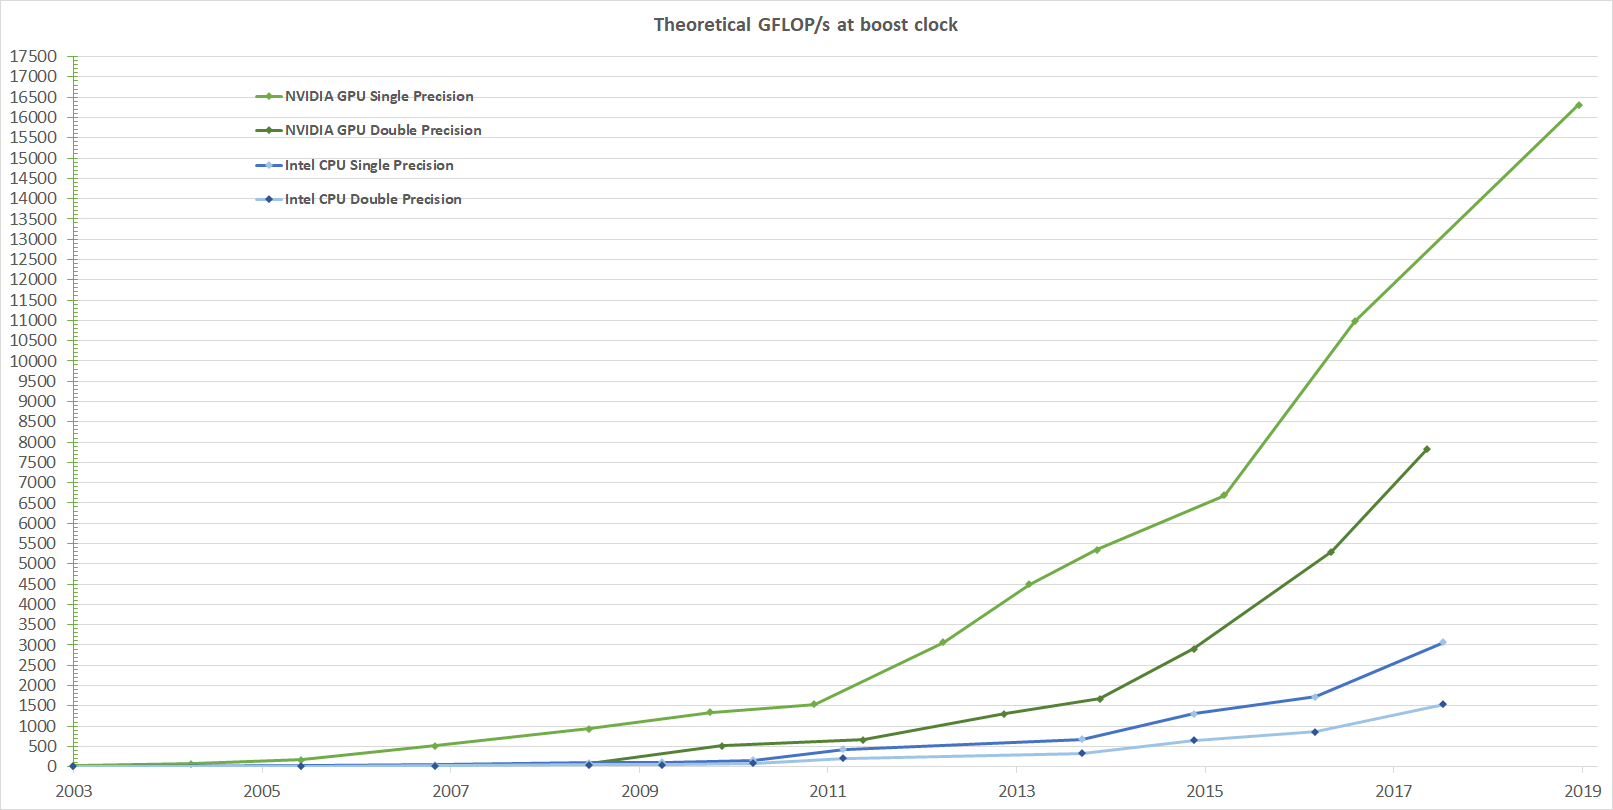
\includegraphics[width=0.8\textwidth]{GPUspeed.png}
    \caption{CPU和GPU浮点运算比较}
    \label{fig:chap1:GPUspeed}
  \end{figure}

\section{研究现状与进展}
  本节介绍SAR图像舰船检测方法研究与进展,包含了单极化SAR图像舰船检测与极化SAR图像舰船目标检测。
\subsection{单极化SAR图像目标检测}
    通常星载SAR系统可以对大范围海面进行成像,对于原始单通道SAR图像数据,舰船目标检测主要包含了以下
    几个过程:海陆分割,截取含有潜在目标的候选检测区域,使用目标检测算法鉴别候选区域中的
    舰船像素与杂波像素~\cite{article}。目前大多数检测算法都是依据舰船目标与海面后的向散射特性的差异来进行
    鉴别。舰船目标包含大量二面角,后向散射系数较高,在强度图像中表现为一块高亮区域,而海杂波则为
    无规则的灰暗斑点噪声的形态。

    在基于幅值的单极化SAR图像舰船目标检测方法中,应用最广泛的为基于恒虚警率(CFAR)的舰船检测方法。CFAR检测方法根据滑动窗选择
    待检测像素周围的海杂波像素,然后按照事先提出的统计分布模型依据选择的海杂波像素去估计杂波分布参数,得到杂波分布
    后根据恒虚警率$P_{FA}$去计算自适应分割阈值$T$,当待检测像素值大于阈值$T$时将该像素判定为舰船像素~\cite{王兆成2017基于单极化}。
    对于恒虚警率舰船检测方法,其检测精度主要受到两个因素的影响,雷达系统本身的参数,如极化模式、入射角等,另一个是成像区域海况条件如风速
    风向等。

    对于海杂波的统计建模方法,Novak\cite{Novak}提出了双参数CFAR检测方法,该方法采用高斯分布对海杂波进行统计建模,实验结果
    表明在低分辨率匀质杂波的条件下,双参数CFAR检测器拥有较好的检测性能。此外研究人员还采用了其他分布模型如瑞利分布、K分布、对数正太分布
    、Weibull分布来描述海杂波分布特性,经实验验证,这些统计模型都可以有效区分SAR图像中的舰船目标与背景杂波~\cite{Carretero2010Statistical}。虽然有很多可供
    选择的统计分布模型,但是在高分辨率的复杂海洋场景中,这些模型对杂波的拟合精度依然不能满足检测要求,于是一些学者提出了非参数化的检测方法。Jiang et al.~\cite{Q2000Automatic}提出了
    概率神经网络(Probability neural newworks, PNN)来估计海杂波的概率密度函数。Gao~\cite{Gao2011A}提出了基于Parzen-window-kernel的检测方法,该方法利用Parzen窗中的
    核函数去逼近真实SAR图像直方图,从而完成对杂波概率密度函数的估计。近些年来一些基于深度学习的方法也被应用到SAR图像目标检测中。Kang~\cite{Miao2017A}将光学图像目标检测网络Faster-RNN
    与CFAR检测器相结合,将Faster-RCNN网络输出的举荐目标区域作为滑动窗的保护区域对CFAR算法改进。实验结果表明,该算法对可以有效提升对SAR图像中尺寸较小的舰船目标的检测能力。



\section{论文内容}

\chapter{极化白化滤波器舰船目标检测}
\label{cha:PWF}

\section{引言}
\label{sec:intro}
在SAR图像中,斑点噪声是影响图像品质的主要因素之一。通常其由一个分辨单元内多个散射体的回波
相干叠加形成。相干斑的存在导致舰船目标检测中的虚警、漏报率提升,从而影响舰船目标检测的性能,
因此相干斑噪声的处理一直被认为是SAR图像处理中最重要的问题。在拥有多极化的SAR数据后,通过
将散射矩阵各个通道信息进行融合,提取极化特征,可以获取相干斑抑制的重构图像。通常图像SPAN即
散射总功率为最基本的极化特征,相较于单通道SAR图像,其可以显著的减少SAR图像中的相干斑噪声。在本章中
采用了重构图像的标准差s与均值m比进行相干斑噪声的衡量,并证明了极化白化滤波器可以使该比值达到最小,
从而得到最优的重构图像。最后我们采用PWF方法与恒虚警率检测器对极化SAR图像进行处理,结果表明基于极化白化
滤波器的CFAR方法可以有效鉴别海上舰船目标。

\section{海杂波统计特性}
    此节采用复高斯模型来描述海杂波的数学统计特性,包含三个通道的极化散射矢量描述如下
    \begin{equation}
      {\bf{X}}{\rm{ = }}\left[ {\begin{array}{*{20}{c}}
        {{{\bf{S}}_{hh}}} \\
        {{{\bf{S}}_{hv}}} \\
        {{{\bf{S}}_{vv}}} 
        \end{array}} \right]   
    \end{equation}
    极化散射矢量中的HH,HV,VV通道满足联合复高斯分布,因此极化散射矢量满足如下的概率密度分布
    \begin{equation}
        f({\bf{X}}) = \frac{1}{{{\Pi ^3}\left| {{\Sigma _c}} \right|}}\exp ( - {{\bf{X}}^H}\Sigma _c^{ - 1}{\bf{X}})
    \end{equation}
    其中${{\Sigma _c}}=E({\bf{X}}{{\bf{X}}^H})$是极化散射矢量的协方差,$H$代表共轭转置,${\rm{E}}( \cdot )$代表求期望。通常假设海杂波
    散射矢量具有零均值即$E({\bf{X}})=0$,当同极化矢量$ {{{\bf{S}}_{hh}}}$与交叉极化矢量${{{\bf{S}}_{hv}}}$间存在耦合时,海杂波极化协方差
    可以描述为以下的形式:
    \begin{equation}
        {\Sigma _c} = {\sigma _{hh}}\left[ {\begin{matrix}
   1 & 0 & {\rho \sqrt \gamma  }  \\ 
   0 & \varepsilon  & 0  \\ 
   {{\rho ^*}\sqrt \gamma  } & 0 & \gamma   \\ 
   \end{matrix}} \right]
    \end{equation}
    在上式中$*$代表共轭转置

    \begin{equation}
        \begin{array}{l}
        {\sigma _{hh}} = E({\left| {S_{hh}} \right|^2})\\
        \varepsilon  = \frac{{E({{\left| {S_{hv}} \right|}^2})}}{{E({{\left| {S_{hh}} \right|}^2})}}\\
        \gamma  = \frac{{E({{\left| {S_{vv}} \right|}^2})}}{{E({{\left| {S_{hh}} \right|}^2})}}\\
        \rho  = \frac{{E(S_{hh} \cdot S_{vv})}}{{\sqrt {E({{\left| {S_{hh}} \right|}^2})E({{\left| {S_{vv}} \right|}^2})} }}
        \end{array}
    \end{equation}

\section{极化白化滤波器}
    利用HH,HV,VV三个通道的极化信息构建最优图像,采用重构图像的标准差$s$与均值$m$之比进行斑点噪声的度量。下面将
    证明极化白化滤波器可以使得标准差与均值的比值达到最小。

    \begin{equation}
        \label{equ:chap3:measure}
        \frac{s}{m} = \frac{{\sigma (y)}}{{E(y)}}
    \end{equation}

    上式中随机变量$y$代表重构的图像像素,当给定SAR图像HH、HV、VV通道极化信息后,通过下式来重建斑点
    抑制图像

    \begin{equation}
        \label{equ:chap3:construct}
        y = {{\bf{X}}^H}A{\bf{X}}
    \end{equation}
    在式\ref{equ:chap3:construct}中,权重矩阵A为厄米共轭且正定,为了找到最优权重矩阵$A^*$,将式
    \ref{equ:chap3:measure}做如下变换,式\ref{equ:chap3:trans}中,$\lambda_1, \lambda_2, \lambda_3$为
    矩阵${\Sigma _c}A$的特征值,因此寻找最优权重矩阵的问题被转化为寻找特征值$\lambda_1, \lambda_2, \lambda_3$
    使得$s/m$比值达到最小。显然当矩阵$\Sigma_cA$为单位阵特征值$\lambda_1=\lambda_2=\lambda_3$时,该比值达到最小。
    因此$A^*$=$\Sigma_c^{-1}$被称作极化白化滤波器。


    \begin{equation}
        \label{equ:chap3:trans}
        \begin{array}{*{20}{c}}
            {\sigma (y) = tr{{({\Sigma _c}A)}^2} = \sqrt {\mathop \Sigma \limits_{i = 1}^3 {\lambda _i}^2} }\\
            {E(y) = tr({\Sigma _c}A) = \mathop \Sigma \limits_{i = 1}^3 {\lambda _i}}\\
            {\frac{s}{m} = \frac{{\sqrt {\mathop \Sigma \limits_{i = 1}^3 {\lambda _i}^2} }}{{\mathop \Sigma \limits_{i = 1}^3 {\lambda _i}}}}
        \end{array}
    \end{equation}

    获得极化白化滤波器后,通过式\ref{equ:chap3:recon}得到最小化相干斑重构图像。从式\ref{equ:chap3:recon}
    可以看出相干斑抑制图像是对${{{\left| {{S_{hh}}} \right|}^2}}$,${{{\left| {{S_{hv}}} \right|}^2}}$,
    ${{{\left| {{S_{vv}}} \right|}^2}}$三个通道进行优化权重求和得到的强度图像。相较于单极化强度图像,极化白化
    滤波器提供了$4.8dB$的相干斑噪声抑制。

    \begin{equation}
        \label{equ:chap3:recon}
        y = \frac{{{{\left| {{S_{hh}}} \right|}^2}}}{{{\sigma _{hh}}(1 - {{\left| \rho  \right|}^2})}} + \frac{{{{\left| {{S_{vv}}} \right|}^2}}}{{{\sigma _{hh}}(1 - {{\left| \rho  \right|}^2})\gamma }} + \frac{{{{\left| {{S_{hv}}} \right|}^2}}}{{{\sigma _{hh}}\varepsilon }} - \frac{{2{\mathop{\rm Re}\nolimits} (\rho  \cdot {S_{hh}}^* \cdot {S_{vv}})}}{{{\sigma _{hh}}(1 - {{\left| \rho  \right|}^2})\sqrt \gamma  }}
    \end{equation}

   采用实验数据来验证PWF相干斑抑制效果,实验数据选择的是C波段多极化大连港的原始图像数据,所截取图像为1000x1000的
   海洋场景,在自适应极化白化滤波器方法中,使用大小为31x31的滑动窗选择海杂波像素来计算协方差矩阵,下表为原图像SPAN方法,PWF方法
   与APWF(自适应极化白化滤波器)方法处理后图像的标准差与均值比

  \begin{table}[htb]
  \centering
    \begin{minipage}[t]{0.8\linewidth} % 如果想在表格中使用脚注,minipage是个不错的办法
    \caption[不同强度图像s/m比值]{HH、SPAN与APWF强度图像标准差与均值比}
    \label{tab:template-files}
      \begin{tabularx}{\linewidth}{lXXX}
        \toprule[1.5pt]
        {\heiti 滤波方法} & {\heiti HH强度图像} & {\heiti SPAN强度图像} & {\heiti APWF强度图像}\\ \midrule[1pt]
        s/m & 2.02 & 2.25 & 11.24 \\
        \bottomrule[1.5pt]
      \end{tabularx}
    \end{minipage}
\end{table}

  不同强度图像如图\ref{fig:chap3:intensity}所示,从图像结果中可以看到,SPAN强度图像与
  APWF强度图像对相干斑都有抑制效果,并且增强了船-海之间的对比对,可以对重构强度图像进行统计
  分析来进一步实施舰船检测。
  \begin{figure}[h]
    \centering
    \subcaptionbox{HH强度图\label{fig:subfig1}}[0.33\textwidth]
      {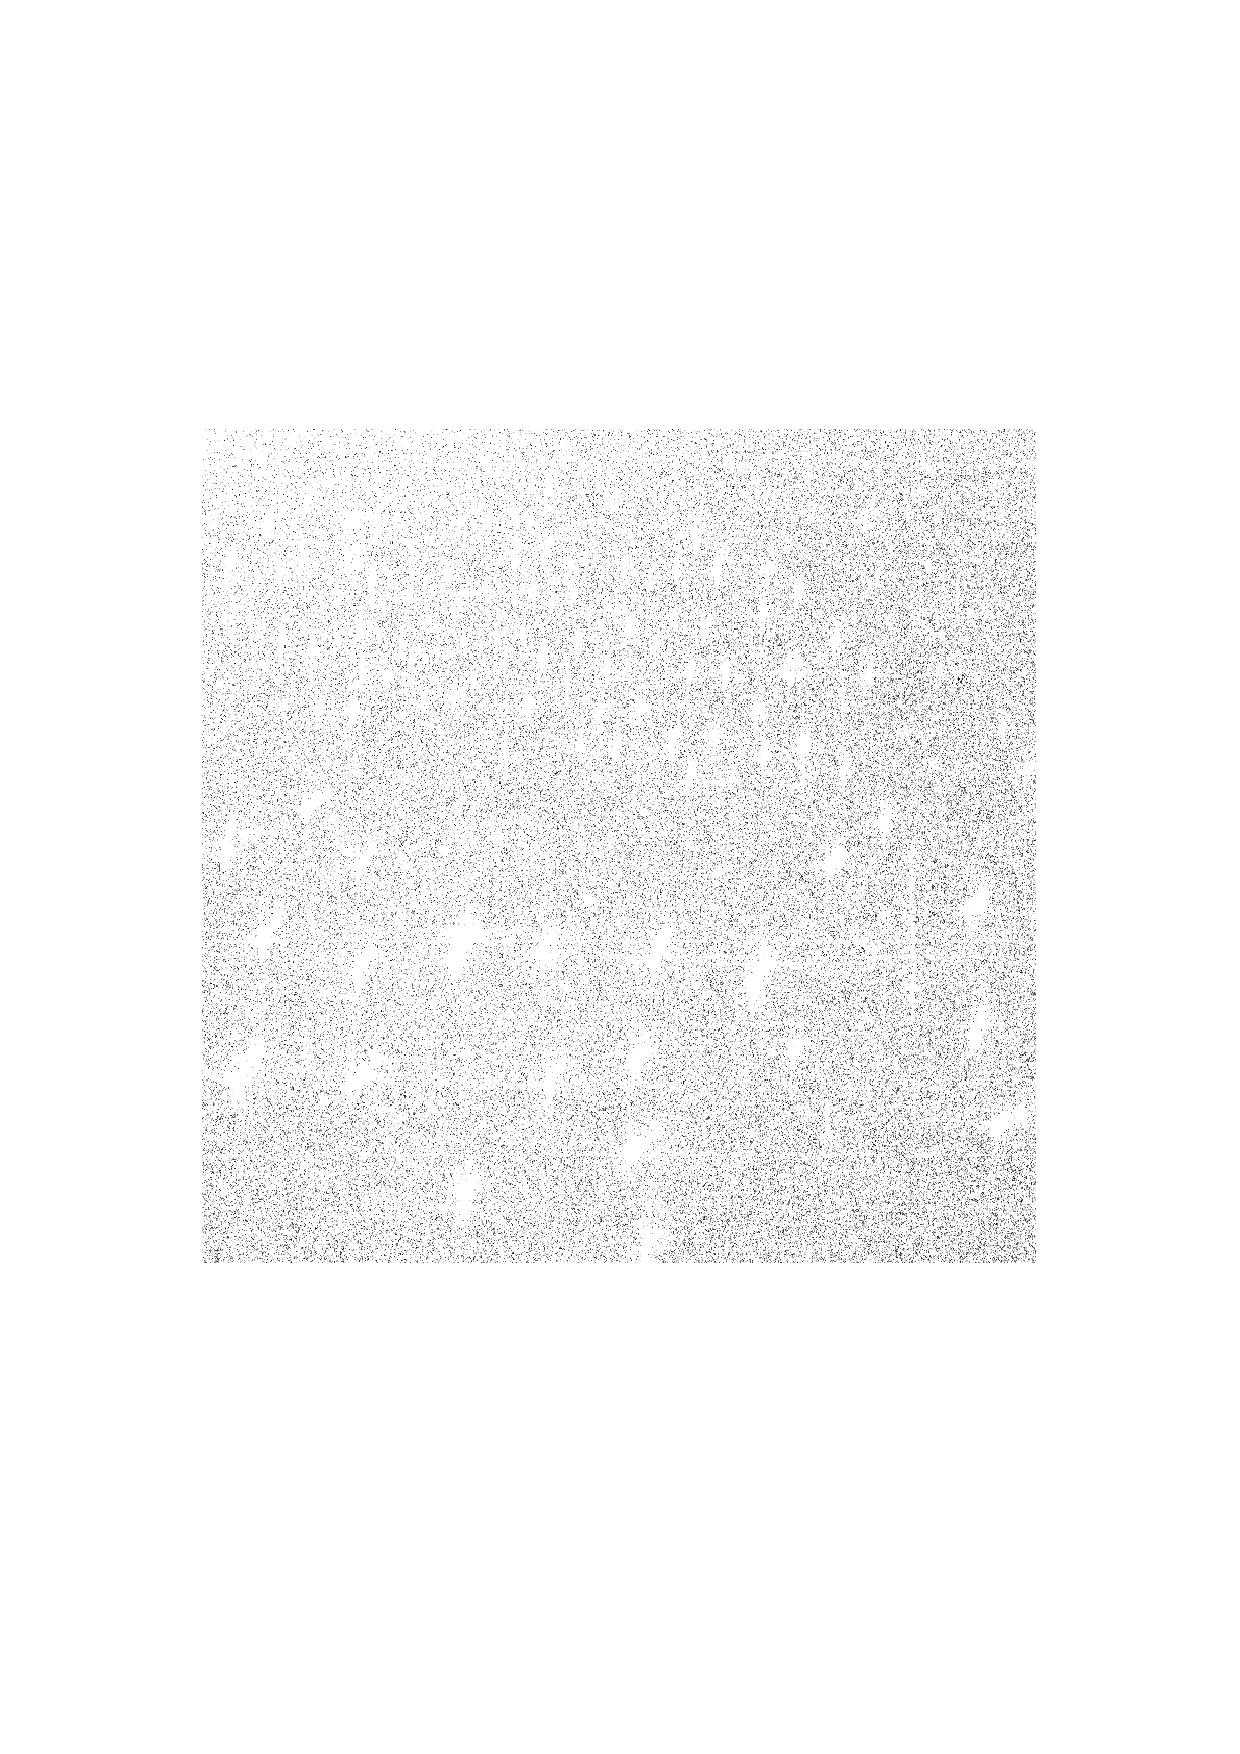
\includegraphics[width=0.33\textwidth]{HH.pdf}}%
    \subcaptionbox{SPAN强度图\label{fig:subfig2}}
        {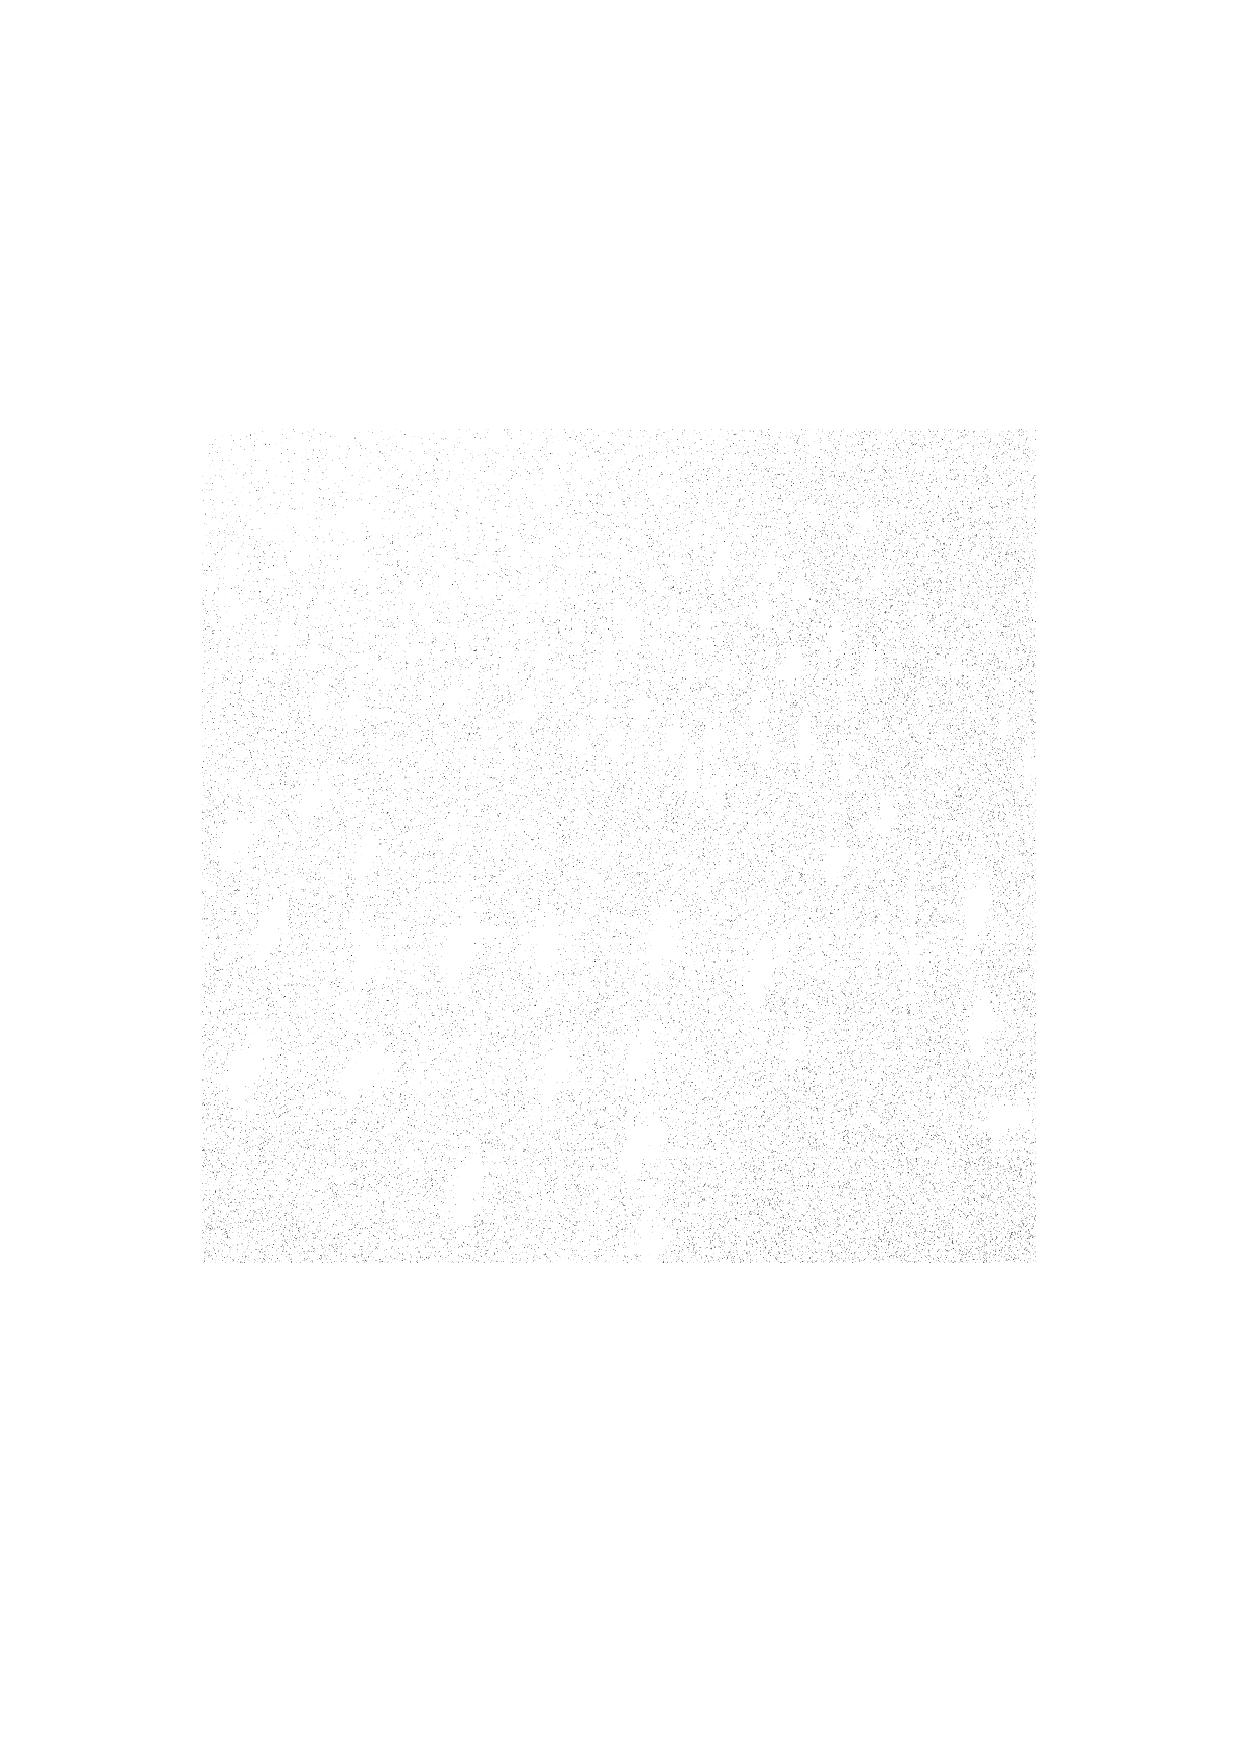
\includegraphics[width=0.33\textwidth]{SPAN.pdf}}
    \subcaptionbox{APWF强度图\label{fig:subfig2}}
        {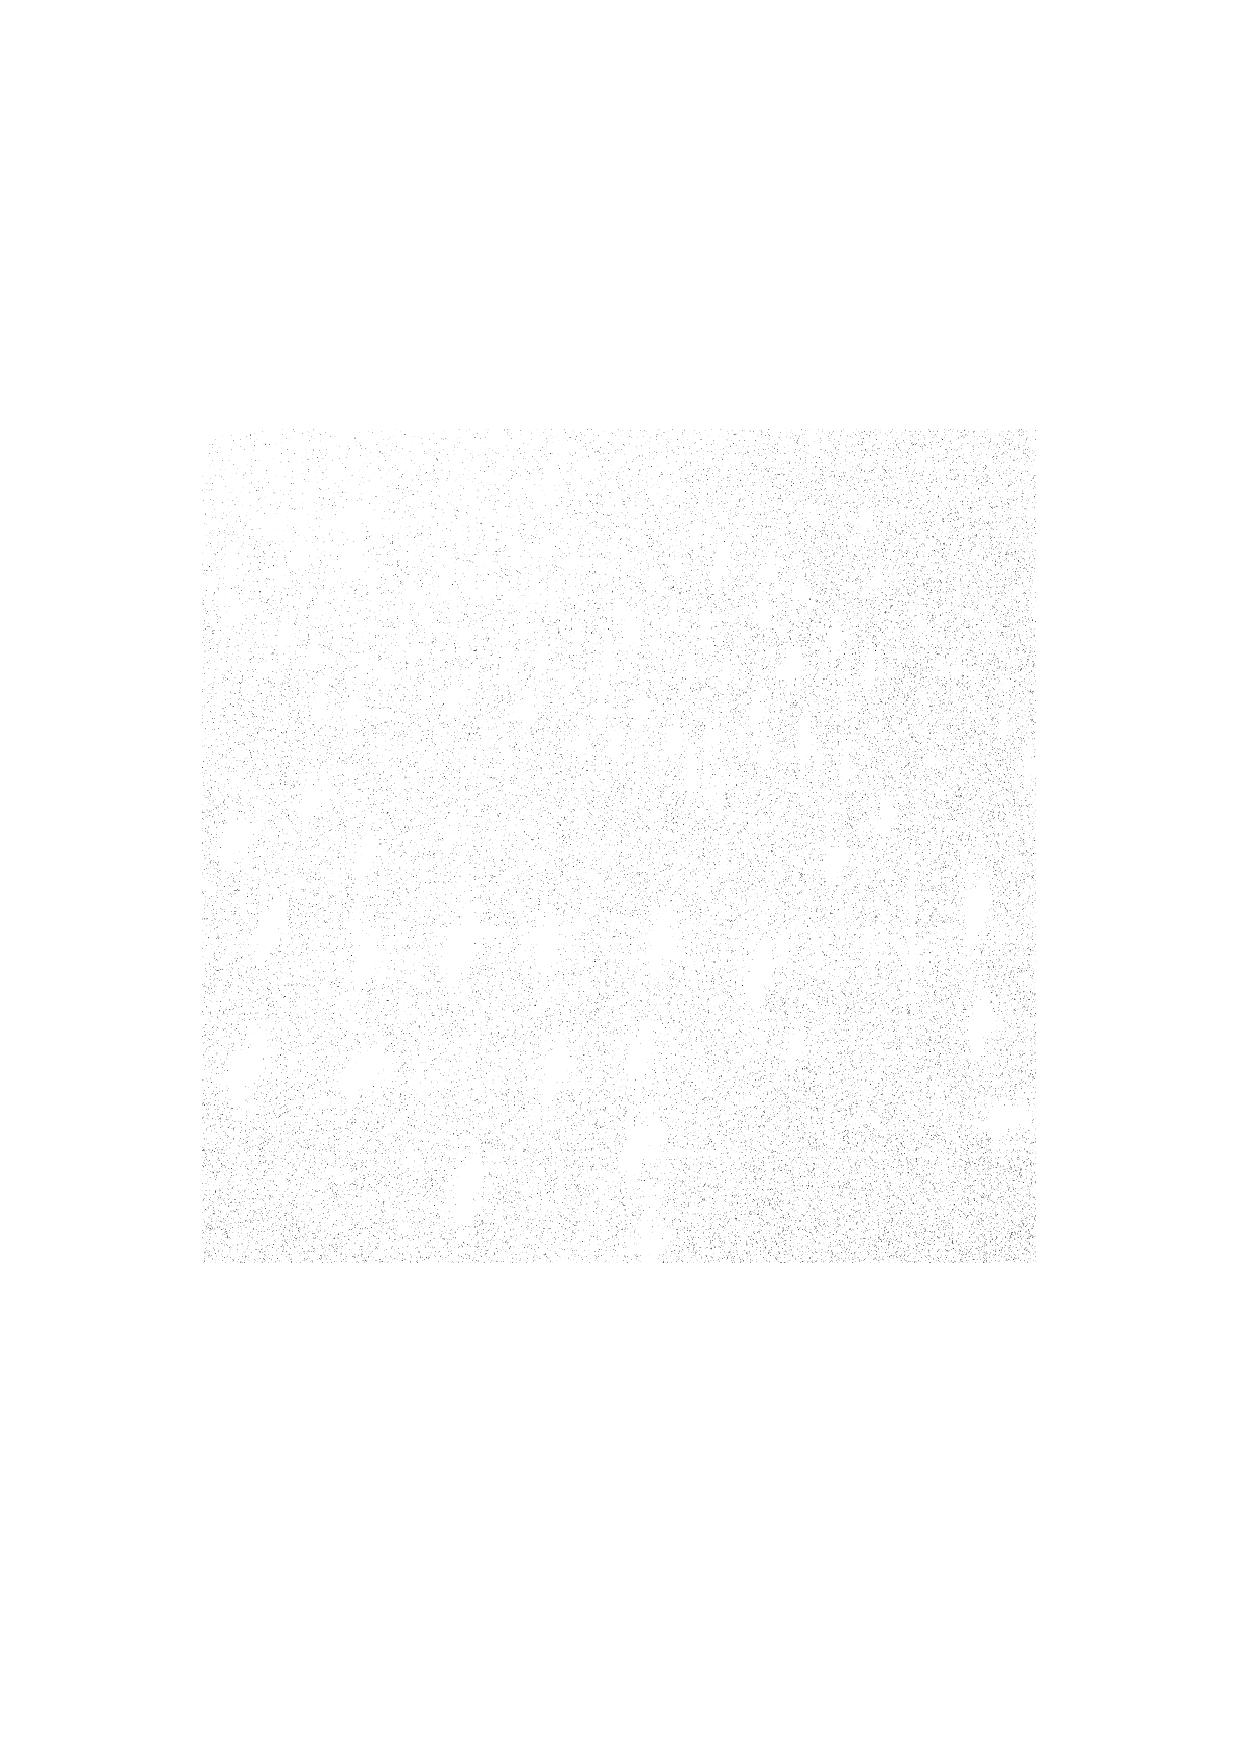
\includegraphics[width=0.33\textwidth]{SPAN.pdf}}
    \caption{HH,SPAN与APWF强度图像}
    \label{fig:chap3:intensity}
  \end{figure}

\section{自适应PWF舰船检测算法}
不同天气条件下的海况不同,因此在SAR图像不同区域的杂波表现差别也很大,为了让算法具有更好的普适性,
采用自适应极化白化滤波器(Adaptive PWF)舰船检测方法。在本章前三节描述了当海杂波散射矢量满足复高斯分布时,
可以采用滑动窗选择局部海杂波散射矢量计算极化白化滤波器参数,并使用该滤波器生成相干斑抑制图像,在文献
[3]中表明,使用自适应极化白化滤波器生成的重构强度图像值满足如下分布:

\begin{equation}
  \label{equ:chap3:pdf}
  {f_y}(y) = {(N)^{N - \rho  + 1}}\frac{{{y^{(\rho  - 1)}}}}{{{{(y + N)}^{N + 1}}}}\frac{{\Gamma (N + 1)}}{{\Gamma (\rho )\Gamma (N - \rho  + 1)}}
\end{equation}
式\ref{equ:chap3:pdf}中,$\rho$为极化散射矢量的维度,$N$为滑动窗内极化散射矢量的个数。当给定恒虚警率
时我们可以轻松的检测阈值,当$N$很大时检测阈值与恒虚警率近似有以下的关系。式\ref{equ:chap3:threshold}中,$T$代表
检测阈值,$P_{FA}$为恒虚警率。

\begin{equation}
  \label{equ:chap3:threshold}
  {P_{FA}} = \exp ( - T)\mathop \Sigma \limits_{k = 0}^{\rho  - 1} \frac{{{T^k}}}{{k!}}
\end{equation}

整个算法流程如Alogrithm~\ref{alg:chap3:APWF}所示,在该算法中要对图像中的所有像素值进行判断,
所以使用的滑动窗的个数等于图像的像素数量。对于大小为N的滑动窗,每一个滑动窗内算法时间复杂度为$O(N)$,
整个算法的时间复杂度为$O(n^3)$, 因此使用滑动窗检测运行时间与滑动窗和原始SAR图像大小有关。当图像或滑动窗尺寸较大
时,整个算法的时效性差不能满足实时检测的要求,所以要在时间方面进行优化。此算法各个滑动窗所对应的自适应极化
白化滤波器参数估计相互独立,因此可以采用并行计算的方式来提高算法的运行效率。

\begin{algorithm}[t]
  \caption{自适应极化白化滤波器舰船检测算法}
  \label{alg:chap3:APWF}
	\KwIn{极化SAR数据,$S_{hh}$,$S_{hv}$,$S_{vv}$}
  \BlankLine
  
  对原始图像边缘根据所选择的滑动窗大小做镜像延拓。

	\ForEach{图像中的像素}{
      从原始SAR图像中根据滑动窗选择海杂波散射矢量$\bf{X}$

      计算自适应极化白化滤波器参数$\Sigma_c$

      根据自适应极化白化滤波器生成重构强度图像值$y$

      依据式\ref{equ:chap3:threshold},采用牛顿迭代法得到检测阈值$T$

      得到检测结果$result = y > T$
	}
  \KwOut{二值舰船检测结果图像$result$}  
 \end{algorithm}

\section{基于GPU的PWF算法实现}

\subsection{GPU算法设计与优化}
 对于APWF舰船检测方法,不同像素对应的自适应极化白化滤波器参数计算过程完全相同,只是通过滑动窗
 选取的海杂波数据不同,因此我们将可并行且计算密集的滤波器参数计算部分放到GPU上去执行。在GPU编程模型中
 ,线程有两个并行的层次分别是网格层次和线程块层次,一个线程块中的线程会作为一个整体被调度到流多处理器上
 去执行。为充分利用GPU硬件资源,将线程块大小设计为32x32即每个线程块中包含1024个线程,网格大小设计为16x16。
 实验中使用的图像大小为1000x1000,故让一个线程块中共1024个线程对应处理SAR图像一行的数据,每个线程通过自身的
 二维索引和SAR图像中的像素一一对应。

 将线程索引与像素索引对应后,从GPU全局内存(Global Memory)中读取该像素邻域的海杂波数据。在一个线程块内,数据的读取是以线程束的方式进行的。
 一个线程束中包含32个线程,当线程束中线程访问的数据地址在128字节范围内时,该访问可以进行合并。合并访问可以大大
 加快内存访问的速度,提升总线利用效率。因此在算法设计过程中,将全局数据复制到线程私有空间采用行访问的形式可以保证
 线程束中线程访问的地址空间位于128字节段范围内。

  \begin{figure}[H] % use float package if you want it here
    \centering
    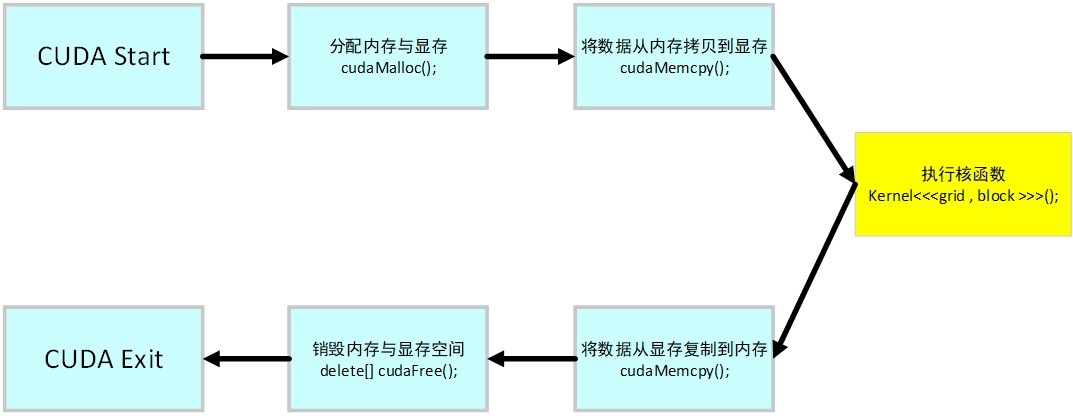
\includegraphics[width=0.8\textwidth]{kernel.jpg}
    \caption{CUDA执行流程}
    \label{fig:chap3:kernel}
  \end{figure}

 核函数的设计,在GPU上所有的线程按照单指令多线程的方式去执行。不同的线程在私有数据空间上去执行相同的指令。对于APWF
 方法,核函数数的主要任务是计算极化白化滤波器参数即海杂波散射矢量的协方差矩阵,协方差矩阵计算主要涉及一个3xN与一个Nx3
 的矩阵相乘,对于该矩阵乘法,采用了动态并行的方式进行了进一步的优化,从当前核函数中创建新的核函数来完并行完成矩阵乘法运算。
 得到滤波器参数后,按照式\ref{equ:chap3:construct}生成重构强度值,并与牛顿迭代法获得的阈值做分割,输出二值检测结果
 图像。
\subsection{多GPU协同}

 多GPU协同APWF方法实现,当多个GPU通过PCIe总线连接时,不同GPU设备之间可以进行通信与同步。多GPU编程中要首先确定
 系统中可用的GPU数量,之后将计算任务合理的分配到各个GPU上。在APWF算法设计中,首先为各个GPU设备分配设备内存,流和事件
 并将SAR图像数据从主机内存拷贝至设备内存。然后依据系统的GPU数量,将原SAR图像进行按行划分并将计算任务分配到不同的GPU流上。
 当流中的核函数执行完成后,将不同GPU上的检测结果复制到主机内存中,作为最终的检测结果。在多GPU编程实现过程中,为了便于
 多GPU之间进行通信,采用了同一虚拟寻址的技术,将所有变量映射到相同的虚拟地址空间中,方便主机和设备进行访问。

 \section{实验结果与加速比测试}

 本次实验在NVDIA TIATN V平台上对APWF舰船检测方法进行测试,图\ref{fig:chap3:resultPWF}为海洋SAR图像检测结果,为了
 衡量SAR图像的检测效果,定义$F_1=\frac{{{N_{tt}}}}{{{N_{fa}} + {N_{gt}}}}$作为评价指标,其中$N_{tt}$为正确检测舰船目标个数,$N_{fa}$
 为虚警的数量,$N_{gt}$为数据船只的真实数量。

 本次实验采用的GPU平台为NVIDIA TiTan V, 相对比的CPU平台为(Intel(R) Core(TM) i9-7920X CPU)处理器,实验所用SAR图像大小为1000x1000
 ,滑动的大小为31,经过多次测试,不同算法消耗时间如表\ref{tab:chap3:timeresult}所示。由测试结果可知对于GPU多线程PWF检测方法
 在检测效率上提升了近32倍,而在多卡的条件下提升了53倍。


  \begin{figure}[h]
    \centering
    \subcaptionbox{SPAN图\label{fig:subfig2}}
        {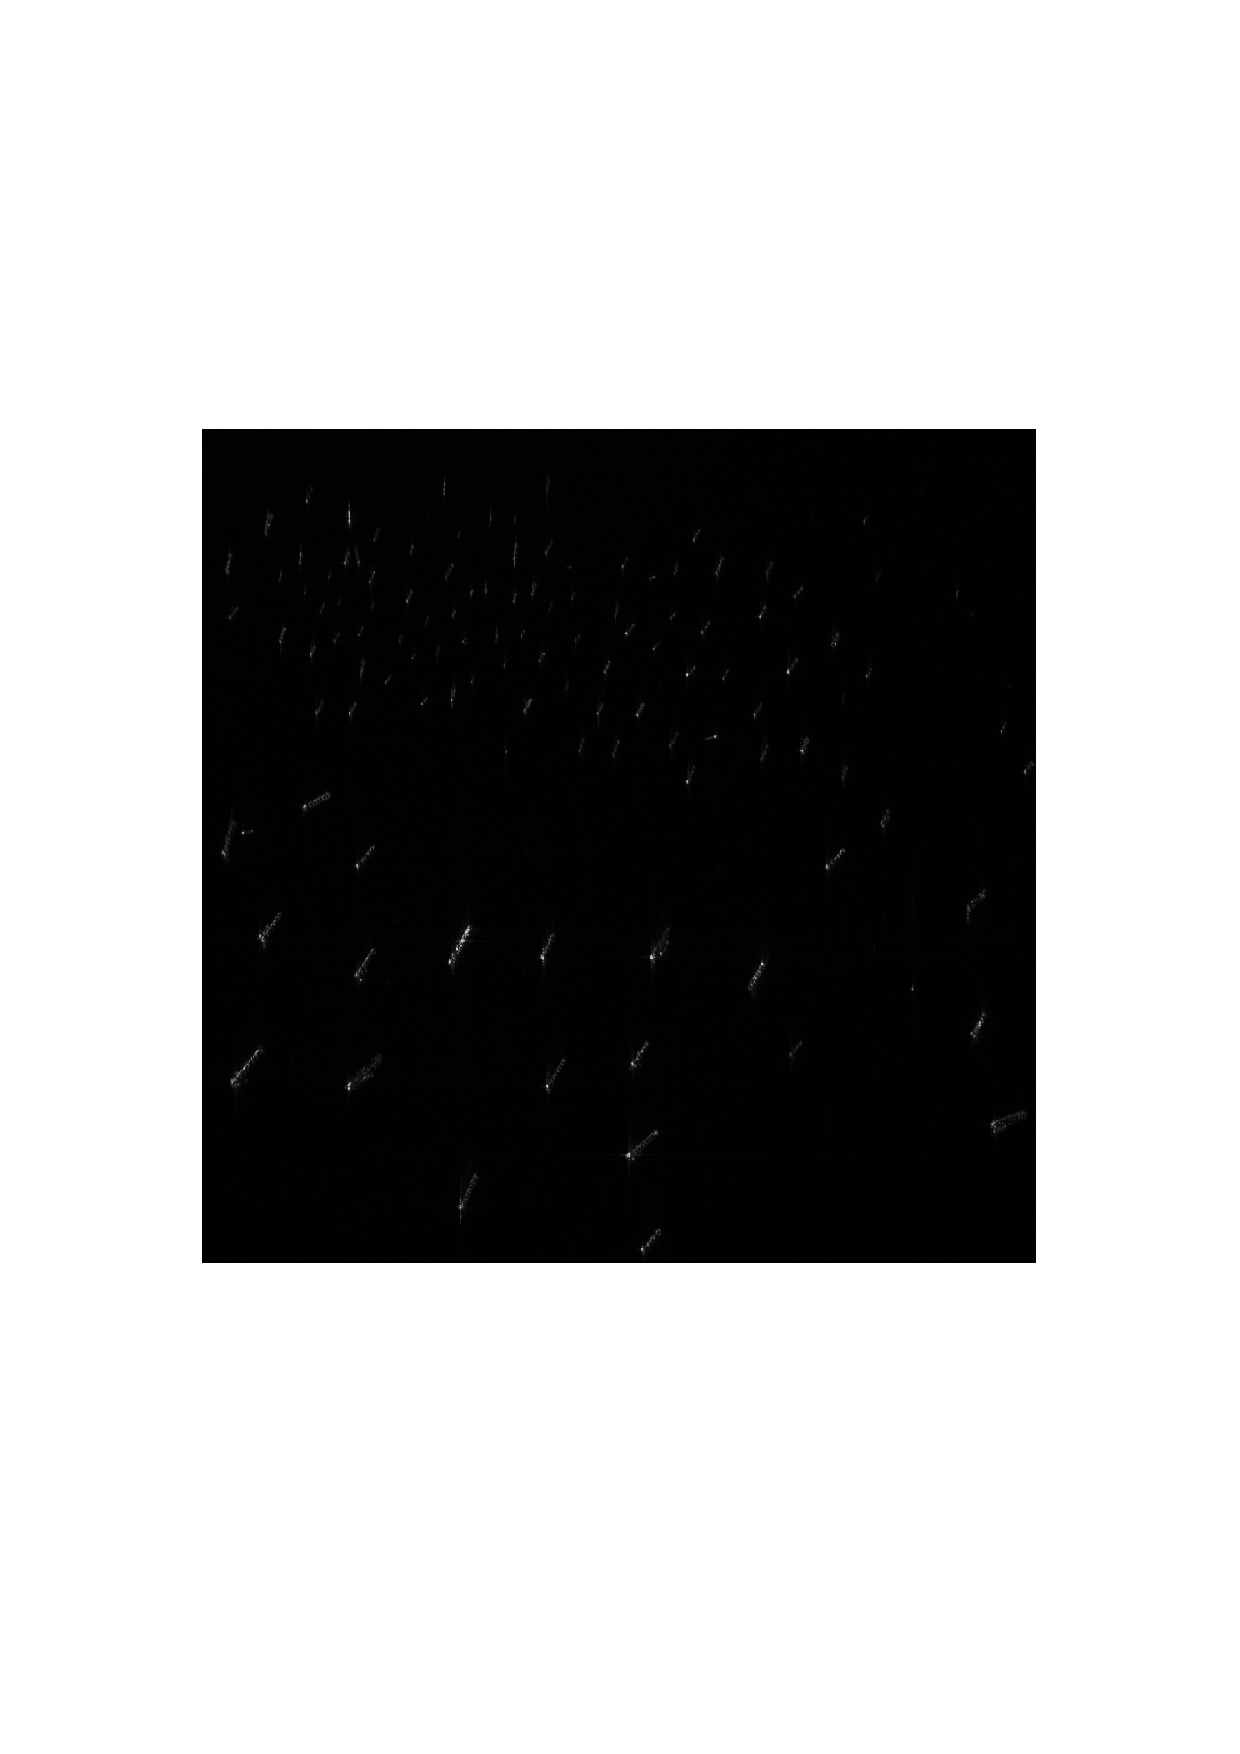
\includegraphics[width=5cm]{resultSPAN.pdf}}
    \subcaptionbox{PWF检测结果\label{fig:subfig2}}
        {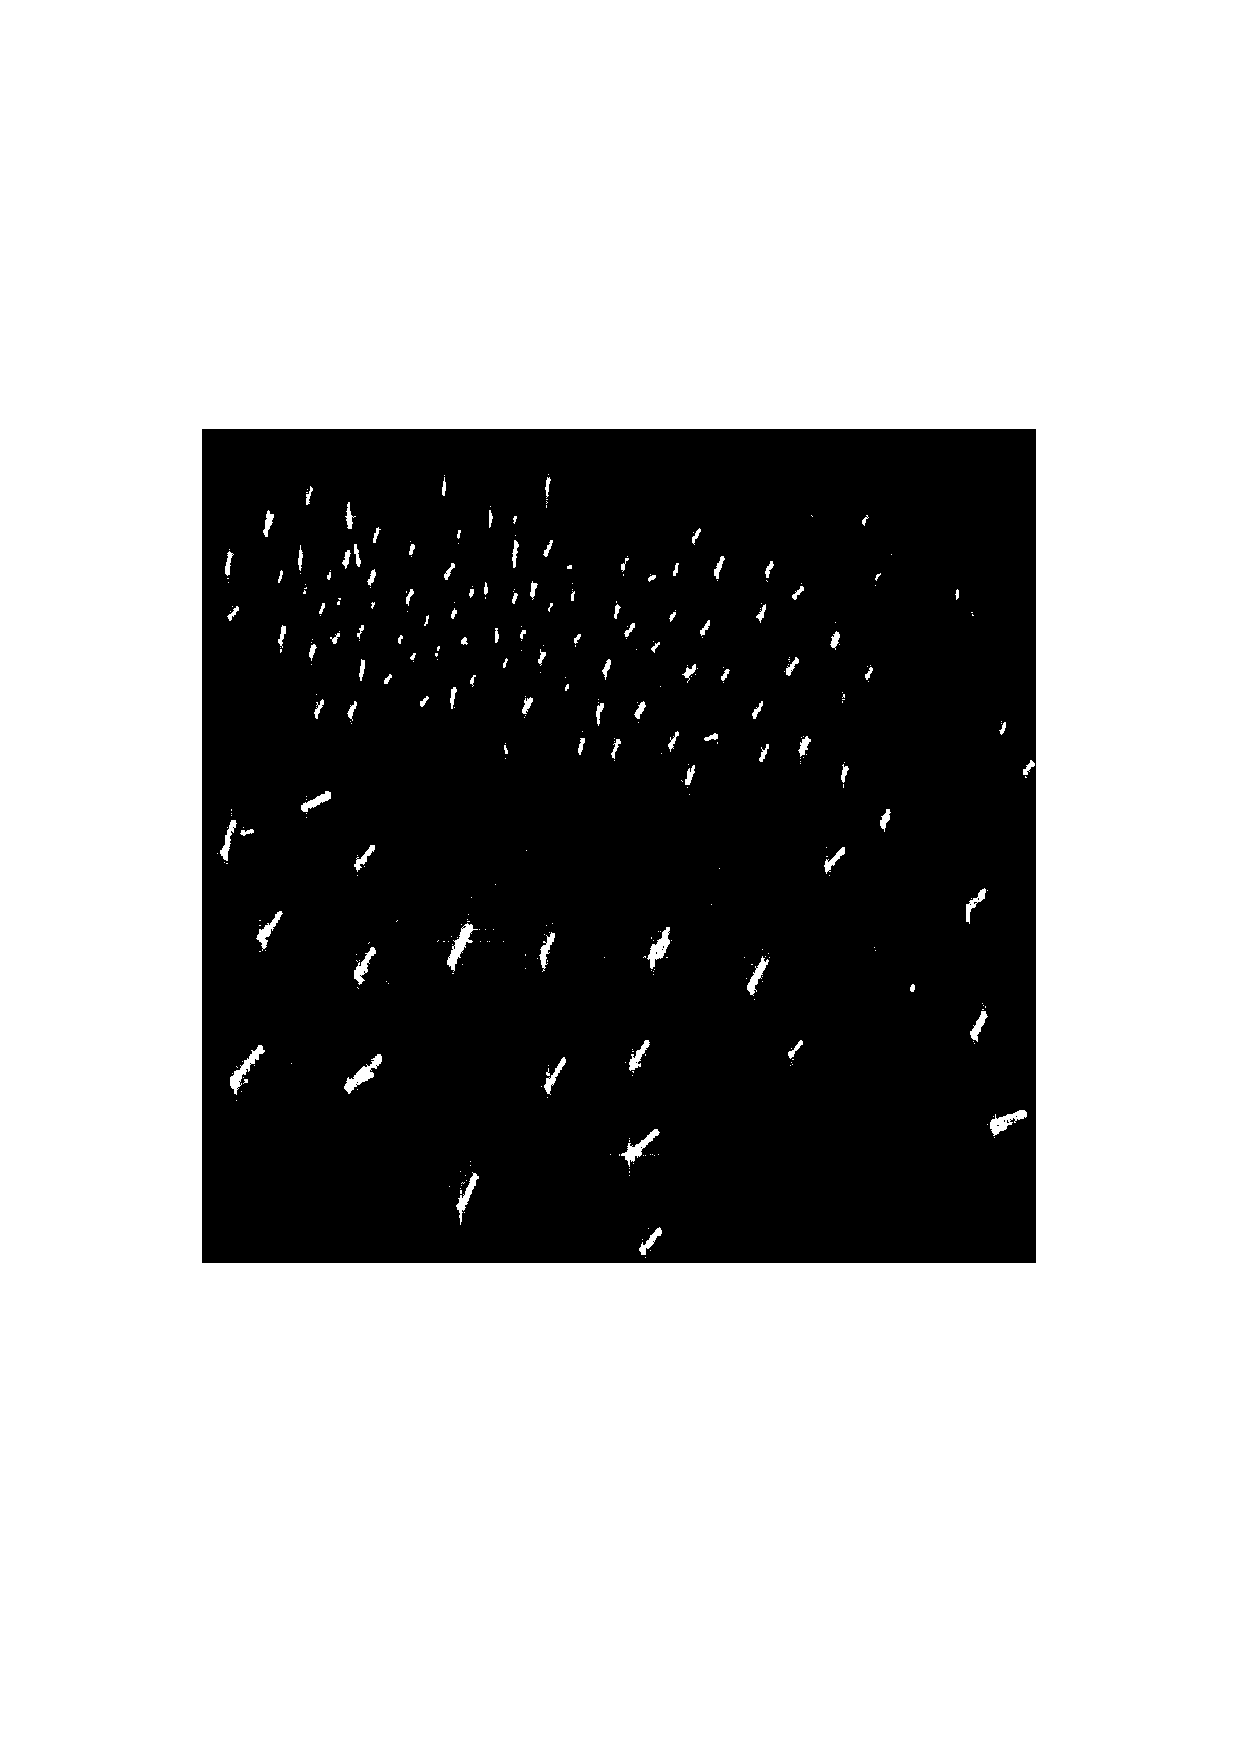
\includegraphics[width=5cm]{resultPWF.pdf}}
    \caption{PWF图像检测结果}
    \label{fig:chap3:resultPWF}
  \end{figure}

  \begin{table}[htb]
  \centering
    \begin{minipage}[t]{1\linewidth} % 如果想在表格中使用脚注,minipage是个不错的办法
    \caption[Adaptive PWF检测结果]{SAR图像极化白化滤波器检测结果}
    \label{tab:chap3:detectresult}
      \begin{tabularx}{\linewidth}{lXXXXXX}
        \toprule[1.5pt]
        {\heiti 检测方法} & {\heiti 船只总数} & {\heiti 总检测数量} & {\heiti 正确检测数量} & {\heiti 虚警数量} & {\heiti 漏报数量} & {\heiti $F_1$}\\ \midrule[1pt]
        PWF & 118 & 123 & 117 & 6 & 1 & 0.943\\
        \bottomrule[1.5pt]
      \end{tabularx}
    \end{minipage}
\end{table}

  \begin{table}[htb]
  \centering
    \begin{minipage}[t]{1\linewidth} % 如果想在表格中使用脚注,minipage是个不错的办法
    \caption[PWF不同平台运行时间]{不同平台PWF算法运行时间}
    \label{tab:chap3:timeresult}
      \begin{tabularx}{\linewidth}{lXX}
        \toprule[1.5pt]
      {\heiti 检测算法} & {\heiti 运行平台} & {\heiti 运行时间/s} \\ \midrule[1pt]
        PWF & (Intel(R) i9-7920X CPU) & 67.4\\
        GPU多线程PWF &  GPU(Titan V) & 2.1 \\
        多卡协同PWF & 2 GPU(Titan V) & 1.27 \\
        \bottomrule[1.5pt]
      \end{tabularx}
    \end{minipage}
\end{table}

\section{小结}
  在本章中,我实现了基于GPU的高性能并行极化白化滤波器SAR图像舰船目标检测算法,本章首先对
  自适应极化白化滤波器检测算法原理进行分析,然后结合GPU架构特点,将计算密集且可并行的滤波器参数计算部分
  放到GPU上去并行执行,并进一步将数据和计算任务分配到多GPU上去执行,对原算法在时间性能上进行优化。实验结果表明,
  相比于串行基于CPU的检测方法,基于GPU的并行检测算法在时间性能上获得了数十倍的提升。



\chapter{基于混合对数正态模型SAR图像目标检测}
\label{cha:LMM}

\section{引言}
\label{sec:chap2:sec1}
在使用恒虚警率的SAR图像目标检测方法中,对海杂波的精准建模是其中至关重要的问题。目前可以有效
对海杂波建模的分布模型有锐利分布,K分布,威布尔分布,对数高斯分布等~\cite{Carretero2010Statistical}。在本章中我采用混合对数正态
模型对强度SAR图像中的海杂波进行建模,实质上对数混合正态模型(lognormal mixture model)等价于强度SAR图像在对数域上的混合
高斯模型\cite{838811},因此可以采用EM方法估计分布参数,得到海杂波概率密度分布后应用牛顿迭代法计算分割阈值输出
检测的结果图像


\section{混合对数正态模型}
\label{sec:chap2:sec2}
  定义强度SAR图像中的像素值$\bf{x}$为一随机变量,当其满足式\ref{equ:chap2:LMM}中的分布时,我们称随机变量$\bf{x}$
  服从包含K个成分的混合对数正态分布。

    \begin{equation}
      \label{equ:chap2:LMM}
      {f_x}(x) = \mathop \Sigma \limits_{i = 1}^K {\alpha _i} \cdot \frac{1}{{\sqrt {2\pi } {\sigma _i}x}}\exp ( - \frac{{{{(\ln x - {\mu _i})}^2}}}{{2{\sigma ^2}}}),x > 0
    \end{equation}
  在式\ref{equ:chap2:LMM}中,$\alpha_i$, $\mu_i$, $\sigma_i(i=1,2,...,K)$为混合对数正态分布参数
  其中$\alpha_i$权重系数满足式\ref{equ:chap2:weigth}所示关系。混合对数正态分布为K个对数正态分布
  加权求和。$\mu_i$,$\sigma_i$为各独立的对数正态分布参数。

    \begin{equation}
      \label{equ:chap2:weigth}
      \sum\limits_{i = 1}^K {{\alpha _i} = 1,{\alpha _i} \ge 0} 
    \end{equation}

  对随机变量$\bf{x}$做形式变换,另$Y=\bf{x}$,我们可以推导出对于随机变量$Y$,其满足的概率密度函数如式\ref{equ:chap2:GMM}所示,显然
  随机变量$Y$满足含有K个分量的混合高斯分布,等价来讲对于强度SAR图像采用混合对数正态模型对海杂波进行建模
  等价于在SAR图像对数强度域上应用混合高斯模型,因此在该建模方法中,首先对强度SAR图像取对数变换到对数域,然后应用混合高斯
  模型描述海杂波的分布。

    \begin{equation}
      \label{equ:chap2:GMM}
        {f_Y}(y) = \mathop \Sigma \limits_{i = 1}^K {\alpha _i} \cdot \frac{1}{{\sqrt {2\pi } {\sigma _i}}}\exp ( - \frac{{{{(y - {\mu _i})}^2}}}{{2{\sigma ^2}}})
    \end{equation}


  \section{海杂波分布参数估计}

      在\ref{sec:chap2:sec2}节表明,混合对数正态分布在强度域与混合高斯分布在对数域上等价,因此混合正态
      分布中的参数计算可以采用目前现有的混合高斯模型参数计算方法。在文献~\cite{6087012}中表明了对于混合高斯模型,最大期望算法
      是一种高效的估计混合高斯分布参数的方法。因此在参数估计中,应用EM算法计算海杂波分布参数。参数迭代更新如式\ref{equ:chap2:paramupdate}
      所示。在该式中$\phi (y|{\mu _k},{\sigma _k})$为均值为$\mu_k$,标准差为$\sigma_k$的高斯分布,$n$为参与估计的杂波像素数量,
      $y$为取对数后的图像强度值。      

    \begin{equation}
      \label{equ:chap2:paramupdate}
      \begin{array}{*{20}{c}}
        {{\mu _k}^{i + 1} = \frac{{\sum\limits_{j = 1}^n {{\gamma _{jk}}{y_j}} }}{{\sum\limits_j^n {{\gamma _{jk}}} }}}\\
        {{\sigma _k}^{{\rm{i}} + 1} = \sqrt {\frac{{\sum\limits_{j = 1}^n {{\gamma _{jk}}({y_j} - {\mu _k}^{i + 1})} }}{{\sum\limits_j^n {{\gamma _{jk}}} }}} }\\
        {{\alpha _k}^{i + 1} = \frac{{\sum\limits_j^n {{\gamma _{jk}}} }}{n}}\\
        {{\gamma _{jk}} = \frac{{{\alpha _k}^i\phi ({y_j}|u_k^i,\sigma _k^i)}}{{\sum\limits_{k = 1}^K {{\alpha _k}^i\phi ({y_j}|u_k^i,\sigma _k^i)} }}}
      \end{array}
    \end{equation}

    受自然条件风速、风向的影响,同一SAR图像不同区域的杂波分布不尽相同,因此采用图\ref{fig:chap2:slide}所示的
    滑动窗进行局部杂波像素的选取,该滑动窗分为三个区域分别为检测像素区域,保护区域,杂波区域。合适大小的保护区域可以减少
    舰船目标像素对杂波统计分布参数估计的干扰。选定杂波像素值后,将其代入到式\ref{equ:chap2:paramupdate}中进行
    海杂波分布参数的迭代估计。

    \begin{figure}[H] % use float package if you want it here
      \centering
      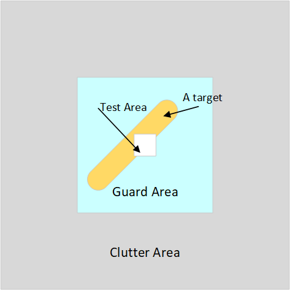
\includegraphics[width=0.5\textwidth]{slide.png}
      \caption{CFAR滑动窗示意图}
      \label{fig:chap2:slide}
    \end{figure}   
\section{应用LMM模型进行CFAR舰船检测}
    当采用混合对数正态模型对海杂波分布进行建模后,根据给定的恒虚警率来实现CFAR方法检测。检测阈值通过
    式\ref{equ:chap2:detecthres}来得到,该式中T为恒虚警率所对应的检测阈值,$f(x)$为采用局部海杂波像素估计
    得到的混合对数正态分布,$F(x)$为$f(x)$对应的累积密度分布函数。我们采用牛顿迭代法来解决这个非线性的
    等式方程,迭代更新公式如式\ref{equ:chap2:newtonupdate}所示,迭代停止的条件为$\left| {{T_{i + 1}} - {T_i}} \right| < \delta$
    当满足迭代精度要求后,最终的检测阈值为${T^*} = {T_{i + 1}}$。

    \begin{equation}
      \label{equ:chap2:detecthres}
      {{\rm{P}}_{FA}} = \int_T^{ + \infty } {f(x)dx = 1 - F(x)}
    \end{equation}

    \begin{equation}
      \label{equ:chap2:newtonupdate}
      {{\rm{T}}_{i + 1}} = {T_i} - \frac{{F({T_i}) + {P_{FA}} - 1}}{{f({T_i})}}
    \end{equation}

    在\ref{sec:chap2:sec2}节,我们证明LMM模型等价于对数域的混合高斯模型,$f(x)$的概率密度函数在对数变换后可表示为式\ref{equ:chap2:GMM}
    的形式。混合高斯分布的累积概率密度函数可以表示为式\ref{equ:chap2:erf}。其中$erf(x)$为误差函数,可以通过查表的方法
    来得到误差函数的值从而减少计算量。

    \begin{equation}
      \label{equ:chap2:erf}
      F(x) = \frac{1}{2}\sum\limits_{i = 1}^K {{\lambda _k}[1 + erf(\frac{{x - {u_i}}}{{\sqrt 2 {\sigma _i}}})]}
    \end{equation}

    综合前几节所述,使用混合对数正态模型的CFAR舰船目标检测流程如算法\ref{alg:chap2:LMM}所示

    \begin{algorithm}[t]
      \caption{基于LMM分布的CFAR舰船检测算法}
      \label{alg:chap2:LMM}
      \KwIn{HH通道强度SAR图像}
      \BlankLine
      初始化,将强度图像做对数变换得到对数域强度图像,设置滑动窗的参数。

      \ForEach{图像中的像素}{
          从对数强度图像中根据滑动窗选择海杂波像素值$\bf{y}$

          采用EM迭代算法计算LMM分布参数$\mu_i$,$\alpha_i$与$\sigma_i$

          根据式\ref{equ:chap2:newtonupdate}计算检测阈值$T$

          如果$y(i,j)>T$则该像素点为舰船目标像素点,否则为背景杂波像素点。
      }
      \KwOut{二值舰船检测结果图像$result$}  
    \end{algorithm}

\section{GPU算法优化}
    通常应用滑动窗的SAR图像目标检测方法都面临着计算复杂度高,时间效率低等问题。而滑动窗参数估计是一类典型的
    可以采用并行方式去计算的问题,不同滑动窗之间所用数据和输出结果是相互独立的,没有依赖与调用关系,因此可以
    将滑动穿参数估计部分在GPU多线程上去执行。

    在估计LMM分布参数的过程中,要进行多次迭代并访问杂波像素值来更新分布参数,因此减少此部分数据访存时间可以
    大幅提升算法的运行效率,对于GPU而言总主要有以下几种存储类型,一、二级缓存,寄存器,全局内存,共享内存,纹理内存,
    常量内存。其中一二级缓存为不可编程的存储介质,系统运行时环境会自动分配数据在其上的位置以获得更加优良的性能。对于可编程
    存储介质,通常每个线程的寄存器数量非常有限,因此不适合存储海杂波像素值。而全局内存、常量内存与纹理内存是板上内存,访问延
    迟相较于片上的共享内存要高20~30倍。因此我们选择片上的共享内存作为海杂波像素的高速暂存存储器,通过访问共享内存上的杂波像素,
    可以优化全局内存访问的模式,从而提升核函数的执行速度。

     \begin{figure}[H] % use float package if you want it here
      \centering
      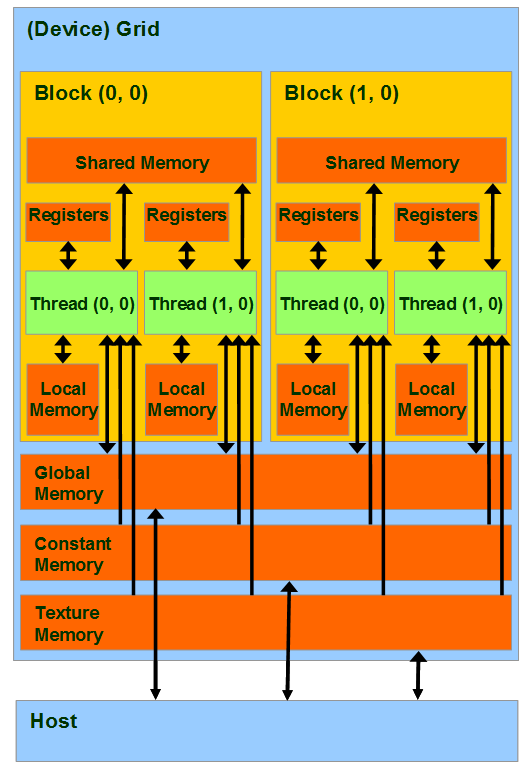
\includegraphics[width=0.5\textwidth]{memory.png}
      \caption{CUDA内存模型}
      \label{fig:chap2:slide}
    \end{figure}   

    共享内存得容量有限,通常为64KB。该存储空间位于流多处理器上类似于CPU的一级缓存,此内存空间被一个线程块中的
    所有线程共享。要合理的设置线程块的大小,避免因共享内存空间过度使用导致活跃线程束减少从而影响程序的执行效率。
    结合滑动窗的大小,我们最终将线程块的大小设置为8x8,将线程网格的大小设置为$(\left\lfloor {\frac{{w + 1}}{8}} \right\rfloor ,\left\lfloor {\frac{{h + 1}}{8}} \right\rfloor )$
    。其中$\left\lfloor {} \right\rfloor $代表向下取整,$w$代表SAR图像的宽度,$h$代表SAR图像的高度。
    
    在分配好线程块与线程网格大小后,每个线程与SAR图像像素索引对应关系为:row = threadIdx.x + blockDim.x * blockIdx.x; column = threadIdx.y + blockDim.y * blockIdx.y;
    之后根据滑动窗,将检测像素所对应的海杂波像素复制到该线程所对应的共享内存内存空间,在EM算法过程中在共享内存中读取杂波像素值进行分布
    的参数更新,当满足参数迭代停止条件后得到LMM分布参数,然后应用牛顿迭代法计算检测阈值$T$,当检测像素值大于阈值$T$时,
    该像素被标记为舰船目标像素。当所有线程执行完毕后,将检测结果从设备内存拷贝至主机内存,进行进一步的分析与处理。

    \begin{figure}[H] % use float package if you want it here
      \centering
      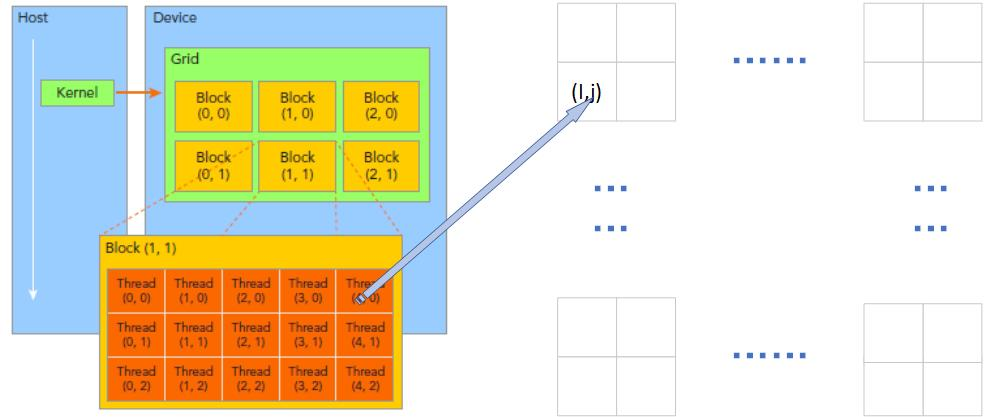
\includegraphics[width=0.9\textwidth]{map.jpg}
      \caption{CUDA线程与检测像素映射关系}
      \label{fig:chap2:slide}
    \end{figure} 

\section{LMM实验结果}
    本次实验中我们使用的是由星载成像雷达系统(SIR-C/X)拍摄的香港维多利亚港的SAR图像数据。SAR图像部分HH通道
    强度图像如图\ref{fig:chap2:source}所示


  \begin{figure}[h]
    \centering%
    \begin{subfigure}{0.4\textwidth}\
      \includegraphics[width=5cm]{HongKong1.png}
    \end{subfigure}%
    \begin{subfigure}{0.4\textwidth}
      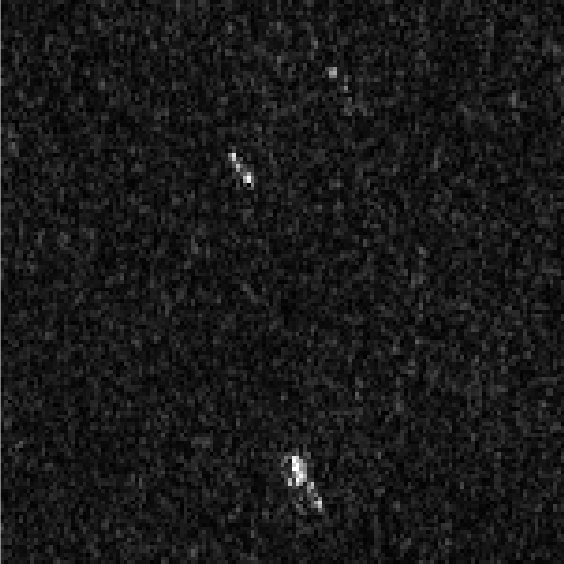
\includegraphics[width=5cm]{HongKong2.png}
    \end{subfigure}

    \begin{subfigure}{0.4\textwidth}
      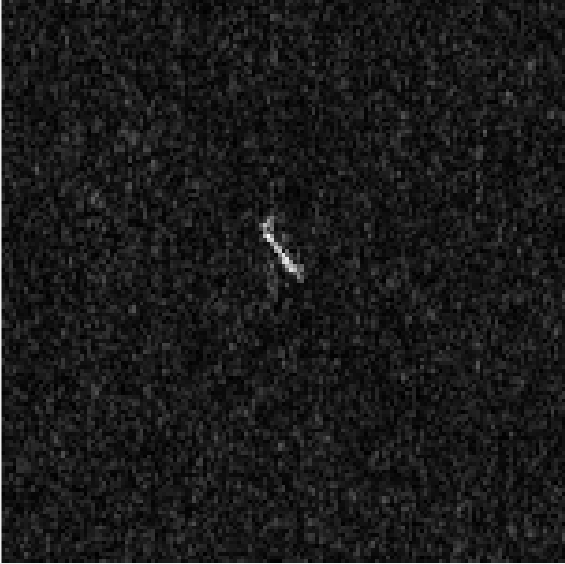
\includegraphics[height=5cm]{HongKong3.png}
    \end{subfigure}%
    \begin{subfigure}{0.4\textwidth}
      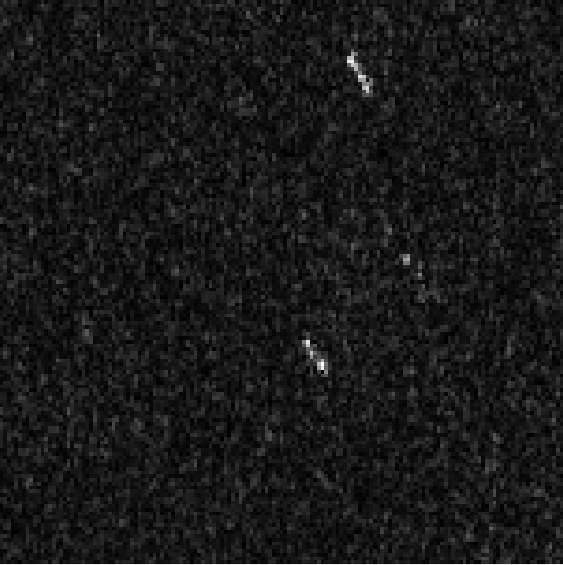
\includegraphics[height=5cm]{HongKong4.png}
    \end{subfigure}   

    \caption{四张SIR-C/XSAR强度图像}
    \label{fig:chap2:source}
  \end{figure}

  在检测中我们设置恒虚警为$1x10^{-5}$,检测结果如图\ref{fig:chap2:detectresult}所示,其中白色区域代表舰船目标像素区域,
  黑色区域代表背景杂波区域,从结果可以看出在给定的虚警率下LMM算法对目标像素与舰船像素作做出了正确的
  分割。本次实验使用的GPU为NVIDIA TITAN V,经过多次实验验证,相较于使用单线程CPU的检测方法,程序运行的时间效率提升了近21倍,
  不同平台运行时间如表所示,原始SAR图像中的舰船数量较少,检测结果中虚警漏报的数量均为0,准确率达到了$100\%$。

  \begin{figure}[h]
    \centering%
    \begin{subfigure}{0.4\textwidth}\
      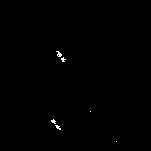
\includegraphics[width=5cm]{HongKong1r.jpg}
    \end{subfigure}%
    \begin{subfigure}{0.4\textwidth}
      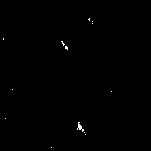
\includegraphics[width=5cm]{HongKong2r.jpg}
    \end{subfigure}

    \begin{subfigure}{0.4\textwidth}
      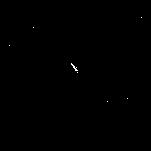
\includegraphics[height=5cm]{HongKong3r.jpg}
    \end{subfigure}%
    \begin{subfigure}{0.4\textwidth}
      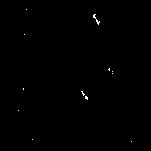
\includegraphics[height=5cm]{HongKong4r.jpg}
    \end{subfigure}   

    \caption{LMM检测结果}
    \label{fig:chap2:detectresult}
  \end{figure}

  \begin{table}[htb]
  \centering
    \begin{minipage}[t]{1\linewidth} % 如果想在表格中使用脚注,minipage是个不错的办法
    \caption[LMM算法时间]{串行与并行LMM算法运行时间对比}
    \label{tab:chap3:timeresult}
      \begin{tabularx}{\linewidth}{lXX}
        \toprule[1.5pt]
        {\heiti 检测算法} & {\heiti 运行平台} & {\heiti 运行时间/s} \\ \midrule[1pt]
        LMM-CFAR(Matlab单线程) & (Intel(R) i7-9750H CPU) & 37.5 \\
        LMM-CFAR(GPU多线程) &  GPU(Titan V) & 1.73 \\
        \bottomrule[1.5pt]
      \end{tabularx}
    \end{minipage}
  \end{table}

\section{小结}
    本章我们实现了基于混合对数正态分布的恒虚警率SAR图像舰船检测方法,在本质上混合对数分布等价于
    强度SAR图像在对数域上的混合高斯分布,因此采用了EM算法与牛顿迭代法得到分布参数与检测阈值。对于滑动窗
    参数估计的部分,我们将其放置在GPU上进行并行计算,并使用延迟更低的共享内存来加快访存速度。相较于传统的
    串行解决方案,本章基于GPU的LMM方法不仅在时间性能获得了显著的提升同时还保证了检测效果的有效性。



\chapter{基于PCDM的极化SAR图像舰船目标检测}
\label{cha:PCDM}

\section{引言}
\label{sec:chap4:sec1}
在第\ref{cha:PWF}章与第\ref{cha:LMM}章,我们实现了基于PWF与LMM模型的舰船检测算法,这两种方法都是
基于图像强度信息进行统计建模以区分舰船目标与背景杂波。然而基于强度或幅值的方法易受海况的影响从而
对海杂波的统计建模不够精确,使得检测性能下降。在本章中我们实现了基于极化协方差差异矩阵的极化SAR
舰船目标检测方法。在极化SAR图像目标检测中,舰船目标点的邻域像素提供了丰富的空间相干信息,极化协方
差矩阵主要度量了待检测像素与其3x3邻域像素的协方差矩阵的差异,基于该极化差异矩阵,我们应用了SPAN检测器得到了
粗略的舰船检测结果。同时我们将PCDM矩阵进行分解提取了新的极化特征基础船高(PSH),通过此极化特征结合SPAN检测器
给出的初步结果进行综合判断得到最终的舰船检测结果。




\section{PCDM理论背景}
\label{sec:chap4:sec2}
\subsection{极化SAR散射表征与SPAN理论}
    通常散射矩阵被用来描述目标散射体的极化信息。在使用水平与垂直极化基的典型极化SAR系统中,复散射矩阵
    定义为如下的形式~\cite{book},其中$S_{HH}$代表了水平发射水平接收的极化信息,当满足互易性的条件时,$S_{HV}=S_{VH}$此时复散射
    矩阵可用三维的复散射矢量$k$式\ref{equ:chap4:kvector}来表示。

    \begin{equation}
        \label{equ:chap4:Smatrix}
        S = \left[ {\begin{array}{*{20}{c}}
        {{S_{HH}}}&{{S_{HV}}}\\
        {{S_{VH}}}&{{S_{VV}}}
        \end{array}} \right]
    \end{equation}

    \begin{equation}
        \label{equ:chap4:kvector}
        k = [{S_{HH}},\sqrt 2 {S_{HV}},{S_{VV}}]
    \end{equation}

    将散射矩阵进行变换可以得到更多散射体的极化信息,如式\ref{equ:chap4:cov}为散射矢量对应的3x3极化协防差矩阵~\cite{Zhang2018Ship}。在该式
    中$\left\langle {} \right\rangle$代表在空间域上求平均,$\left| {} \right|$代表幅度值,$H$代表共轭转置。

    \begin{equation}
        \label{equ:chap4:cov}
        [C] = \left\langle {k \cdot {k^H}} \right\rangle  = \left[ {\begin{array}{*{20}{c}}
        {{C_{11}}}&{{C_{12}}}&{{C_{13}}}\\
        {{C_{21}}}&{{C_{22}}}&{{C_{23}}}\\
        {{C_{31}}}&{{C_{32}}}&{{C_{33}}}
        \end{array}} \right]
    \end{equation}

    在极化协方差矩阵$C$中,将对角线元素之和定义为为后向散射总功率即SPAN,如式\ref{equ:chap4:span}所示。还可以对
    极化协方差矩阵进行分解如式\ref{equ:chap4:decompose}所示~\cite{Liu2010Statistical},其中$\lambda_i$为极化协方差矩阵特征值,$v_i$为$\lambda_i$对应的
    特征向量。
    \begin{equation}
        \label{equ:chap4:span}
        {\rm{SPAN}} = {C_{11}} + {C_{22}} + {C_{33}}
    \end{equation}
    \begin{equation}
        \label{equ:chap4:decompose}
      C = \sum\limits_{i = 1}^3 {{\lambda _i}({v_i} \cdot {v_i}^H)} 
    \end{equation}

    \subsection{极化协方差差异矩阵}
    在计算机视觉领域,LBP特征(局部二值模式)用来描述光学图像中的纹理特征,被广泛应用于人脸检测与目标识别。
    LBP特征是将一个3x3区域内的中心像素值与邻域像素值做比较,并将得到的八位二进制结果重新排列构成一新二进制数值,
    该数值作为此区域中心像素的LBP特征值,如式\ref{equ:chap4:LBP}所示,其中$g_i$表示邻域内第i个像素的灰度值
    $g_c$为中心像素灰度值。$x_c, y_c$表示中心图像坐标。

    \begin{equation}
        \label{equ:chap4:LBP}
        [LB{P_{({x_c},{y_c})}} = \sum\limits_{i = 0}^{n - 1} {{2^{is({g_i} - {g_c})}}} ,s(x) = \left\{ {\begin{array}{*{20}{c}}
        1&{x \ge 0}\\
        0&{x < 0}
        \end{array}} \right.
    \end{equation}

    类比光学图像中的LBP特征~\cite{Lan2017Quaternionic},在极化SAR图像中,采用极化协方差矩阵来描述图像的极化信息。在光学图像中像素的灰度值
    可以通过R、G和B三个通道进行计算得到,而极化协防差矩阵也包含了极化SAR图像的HH、HV和VV通道的信息,但区别是灰度值
    只含有图像的一个特征,而极化协防差矩阵包含了九个极化特征,因此对此模型改进引入极化协方差差异矩阵(PCDM)

    定义${C^{(x,y)}}$为极化SAR图像索引为$x,y$像素处的极化协防差矩阵,接下来计算其3x3邻域上的协方差累积差异$P^{(x,y)}$,
    称$P^{(x,y)}$为极化SAR图像$x,y$处的极化协方差差异矩阵~\cite{张程2018基于},如式\ref{equ:chap4:PCDM}所示,其中$C_{m,n}^{(i,j)}$为
    图像索引$i,j$处协方差矩阵的第$(m,n)$个元素。

    \begin{equation}
        \label{equ:chap4:PCDM}
        P_{m,n}^{(i,j)} = \sum\limits_{\Delta i =  - 1,\Delta j =  - 1}^1 {\left| {C_{m,n}^{(i,j)} - C_{m,n}^{(i + \Delta i,j + \Delta j)}} \right|}
    \end{equation}

    \begin{figure}[H] % use float package if you want it here
      \centering
      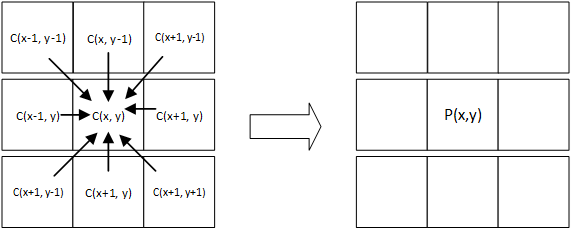
\includegraphics[width=0.9\textwidth]{PCDMCal.png}
      \caption{PCDM矩阵计算示意图}
      \label{fig:chap4:PCDM}
    \end{figure}   
  \section{基于PCDM的舰船目标检测算法}
      前三节我们描述了PCDM可以综合利用待检测像素与其邻域的像素的相干信息,在此基础上我们
      提出了基于极化协方差差异矩阵的舰船检测方法。对于输入的原始极化SAR图像数据,我们首先计算
      每个像素的极化协防差矩阵,然后按照式\ref{equ:chap4:PCDM}计算每个像素对应的极化协方差差异
      矩阵。得到极化协方差差异矩阵$\bf{P}$后,首先对$\bf{P}$矩阵应用SPAN检测器,即当$\rm{SPAN}_{\bf{P}}$>$T_{\rm{SPAN}}$
      时,认定该检测像素为舰船目标像素。

      对PCDM矩阵应用SPAN检测器后输出初步检测结果,为了提升检测的精度,我们进一步提取极化
      协方差差异矩阵的极化特征来区分舰船目标与背景杂波。通常SAR图像目标散射特性可以用极化特征来描述,例如
      极化分解,极化反对称性等极化特征。在文献~\cite{Durden1990The}中提出了pedestal height特征来描述目标的散射特性,
      该极化特征实质上等价于极化协方差矩阵最小特征值与最大特征值的比值。实验表明低海况的背景杂波与方位向模糊像素的
      pedestal height极化特征值比真实的舰船像素要低很多。
       \begin{equation}
          {\rm{PSH = }}\frac{{\left| {{\lambda _3}} \right|}}{{\left| {{\lambda _1}} \right| + \left| {{\lambda _2}} \right|}}
      \end{equation}

      基于极化协方差差异矩阵我们重新计算这些极化特征,并将第二特征值考虑在内,新的极化特征命名为pedestal ship height(PSH)。对于提取的PSH极化特征,应用适当
      的检测阈值,来区分舰船目标与背景杂波像素。整个算法的流程如图\ref{fig:chap4:PCDMalg}所示,算法描述如算法\ref{alg:chap4:PCDMALG}所示

    \begin{figure}[H] % use float package if you want it here
      \centering
      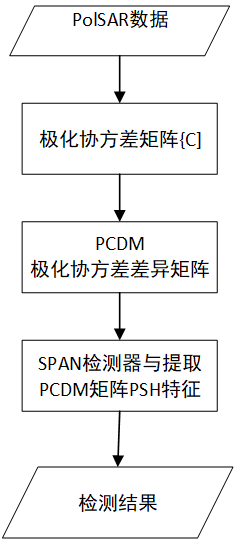
\includegraphics[height=0.5\textwidth]{PCDMalg.png}
      \caption{PCDM检测流程示意图}
      \label{fig:chap4:PCDMalg}
    \end{figure}

    \begin{algorithm}[t]
      \caption{基于PCDM的舰船检测算法}
      \label{alg:chap4:PCDMALG}
      \KwIn{原始极化SAR图像数据}
      \BlankLine
      初始化,计算每个像素的协防差矩阵。

      \ForEach{图像中的像素}{
          根据协方差矩阵计算该像素对应的极化协方差差异矩阵

          计算该极化协方差差异矩阵的SPAN值

          计算极化协方差差异矩阵的基础船高(PSH)极化特征

          将差异矩阵SPAN值与经验阈值作比较,如果$\rm{SPAN}_{PCDM}>T_{SPAN}$,则将该像素为舰船像素。

          将极化特征PSH与经验阈值作比较,如果$PSH_{P(x,y)}>T_{PSH}$,则该像素为舰船像素

      }
      \KwOut{最终舰船检测结果$result$}  
    \end{algorithm}

\section{基于GPU的PCDM算法设计}
      
      前几节描述了基于极化协方差差异矩阵的舰船目标检测算法,在该方法中需要对计算SAR图像每一个像素对应的协方差差异矩阵
      与其极化特征PSH。在该方法中不同像素对应的极化协方差差异矩阵不同,且极化特征估计相互独立,因此将对每个像素的检测
      操作一一对应到GPU上的每个线程。

      线程模块大小设计,本次实验的原始SAR图像数据大小为1000x1000,线程块中的线程以32个为一组进行调度,为充分利用流多处理器
      资源,将线程块大小设计为32x32。考虑到GPU同时并发线程数量的限制与全局内存空间容量,将线程网格大小设计为16x16,对于线程块中的线程
      通过其二维线程索引(threadIDx)与原始SAR图像上的列一一对应,使用线程块索引(blockIDx)与原始SAR图像的行去对应。
      我们设计的线程网格数量为256小于原始SAR图像的行数,因此对SAR图像的检测操作将被分配到四个内核中去执行。内核中的线程通过
      内核序号来找到自己对应的SAR图像行索引,四个内核被装载到同一CUDA流中在GPU上被顺序调度。线程内存空间设计,在CUDA架构中
      不能在核函数中去动态声明较大的内存区域,因此需要在内核执行前由主机分配好线程内存池,然后线程根据自身索引与给定的线程空间大小去找到
      本线程私有内存空间的起始地址。线程内存空间分析,对于PCDM方法,要存储九个像元的散射矩阵信息、协方差矩阵信息与中心像元的极化协方差
      差异矩阵,综合考虑PCDM矩阵计算特征值等其他计算开销,最终我们一个线程所占有的内存空间设置为8192B。

      内核函数的设计,首先计算本线程所对应的二维索引,将该二维索引与其3x3邻域对应的SAR图像数据从全局内存复制到
      线程私有的内存空间中,之后计算这九个像元所对应的协方差矩阵并调整为9x9大小,该矩阵每一列代表各像元的协方差
      矩阵元素。将该矩阵的第五列即中心像素的协方差矩阵与其他列依次做差求绝对和得到极化协方差差异矩阵。得到PCDM矩阵后,首先对
      该矩阵应用SPAN检测器,即计算矩阵对角线元素之和并与经验阈值做比较,当该SPAN值大于经验阈值时,将该像素判别为舰船像素。
      接下来计算极化协方差差异矩阵的PSH极化特征,该特征为PCDM矩阵最小特征值与其他两个特征值绝对值之比,因此问题转化为
      计算极化协方差差异矩阵特征值的问题。PCDM矩阵为实对称矩阵,计算其特征值采用雅克比迭代的方式,迭代过程的矩阵更新
      公式如式\ref{equ:chap4:jacobian}所示,其中$\varphi$通过选择矩阵非对角绝对值最大元素计算得到。具体的算法流程为
      算法\ref{alg:chap4:jacobianeigen}所示。得到矩阵的特征值后计算PSH极化特征的大小并与经验阈值做比较,如果PSH值大于
      经验阈值,则判断该像素为舰船目标像素。当GPU上所有线程核函数执行结束后,主机将检测结果从设备内存拷贝至主机内存,结合
      OpenCV进行图像显示,并保存检测结果。

       \begin{equation}
           \label{equ:chap4:jacobian}
            \begin{array}{*{20}{c}}
            {\left\{ {\begin{array}{*{20}{c}}
            {a_{pp}^{i + 1} = a_{pp}^i{{\cos }^2}\varphi  + a_{qq}^i{{\sin }^2}\varphi  + 2a_{pq}^i\cos \varphi \sin \varphi }\\
            {a_{qq}^{i + 1} = a_{pp}^i{{\cos }^2}\varphi  + a_{qq}^i{{\sin }^2}\varphi  - 2a_{pq}^i\cos \varphi \sin \varphi }\\
            {a_{pq}^{i + 1} = a_{qp}^{i + 1} = \frac{1}{2}(a_{qq}^i - a_{pp}^i)\sin 2\varphi  + a_{pq}^i\cos 2\varphi }
            \end{array}} \right.}\\
            {\left( {\begin{array}{*{20}{c}}
            {a_{pn}^{i + 1}}\\
            {a_{qn}^{i + 1}}
            \end{array}} \right) = \left( {\begin{array}{*{20}{c}}
            {\cos \varphi }&{\sin \varphi }\\
            { - \sin \varphi }&{\cos \varphi }
            \end{array}} \right)\left( {\begin{array}{*{20}{c}}
            {a_{pn}^i}\\
            {a_{qn}^i}
            \end{array}} \right),n \ne p,q}\\
            {\left( {\begin{array}{*{20}{c}}
            {a_{mp}^{i + 1}}\\
            {a_{mq}^{i + 1}}
            \end{array}} \right) = \left( {\begin{array}{*{20}{c}}
            {\cos \varphi }&{\sin \varphi }\\
            { - \sin \varphi }&{\cos \varphi }
            \end{array}} \right)\left( {\begin{array}{*{20}{c}}
            {a_{mp}^i}\\
            {a_{mj}^i}
            \end{array}} \right),m \ne p,q}\\
            {a_{mn}^{i + 1} = a_{nm}^{i + 1} = a_{mn}^i,m \ne p,q;n \ne p,q}
            \end{array}
       \end{equation}

       \begin{equation}
           \label{equ:chap4:rotationangle}
           \tan 2\varphi  = \frac{{ - 2{a_{pq}}}}{{{a_{qq}} - {a_{pp}}}}
       \end{equation}

    \begin{algorithm}[htb]
      \caption{雅克比迭代计算矩阵特征值}
      \label{alg:chap4:jacobianeigen}
      \KwIn{实对称矩阵$\bf{A}$}
      \BlankLine
      初始化特征向量为单位阵。

      \While{$\bf{A}$非主对角元素绝对值<给定阈值}{

        在$\bf{A}$的非主对角元素中找到最大元素值为$a_{pq}$

        用式\ref{equ:chap4:rotationangle}计算旋转角度$\varphi$

        用式\ref{equ:chap4:jacobian}来对矩阵$\bf{A}$中的元素进行更新
          
      }

      将矩阵特征值按照从大到小的顺序进行排序
      \KwOut{矩阵$\bf{A}$的特征值}  
    \end{algorithm}

\section{PCDM算法检测结果}
    在本次实验中我们使用的是Radarsat-2拍摄的远洋极化SAR数据,通常舰船目标相对于海平面的后向散射系数更高,具有更高的散射回波
    功率,因此舰船SAPN强度像素值要高于海杂波像素。在PCDM方法中充分利用了检测像素与其邻域像素的空间相干关系,因此基于PCDM的SPAN图像可以提升船海之间的差异度,
    有着更强的舰船与海杂波的区分能力,图\ref{tab:chap4:detectresult}所示的为SAR局部图像切片的SPAN图像与PCDM SPAN图像的对比。从实验结果
    上表明,基于PCDM的舰船像素与海杂波像素SPAN值的对比度相较于基于协方差矩阵的SPAN值的对比度更加明显。因此我们选取PCDM SPAN最大值与最小值差
    的千分之五作为分割阈值,从而区分舰船目标与背景杂波。

  \begin{figure}[h]
    \centering
    \subcaptionbox{PCDMSPAN图\label{chap4:fig:subfig2}}
        {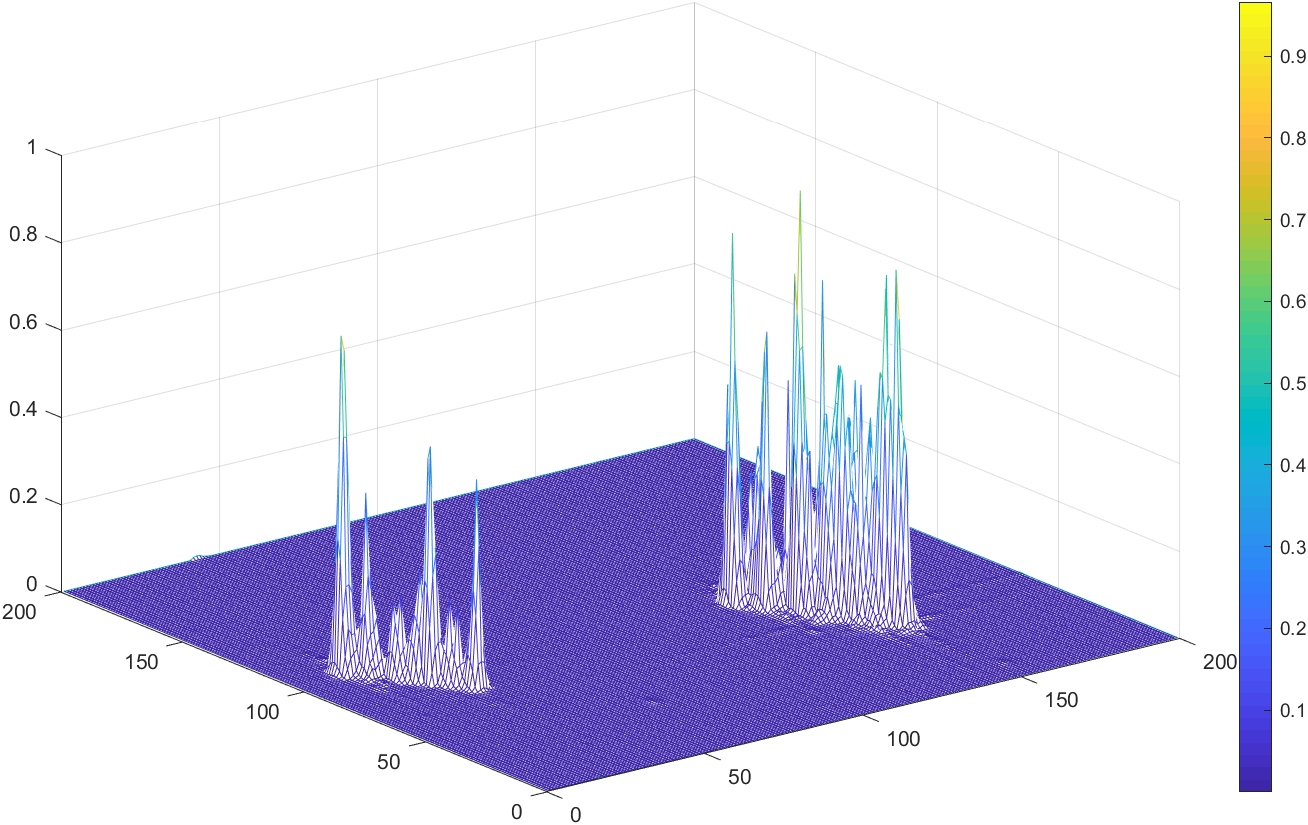
\includegraphics[width=9cm]{PCDMSPAN.png}}
    \subcaptionbox{SPAN图像\label{chap4:fig:subfig2}}
        {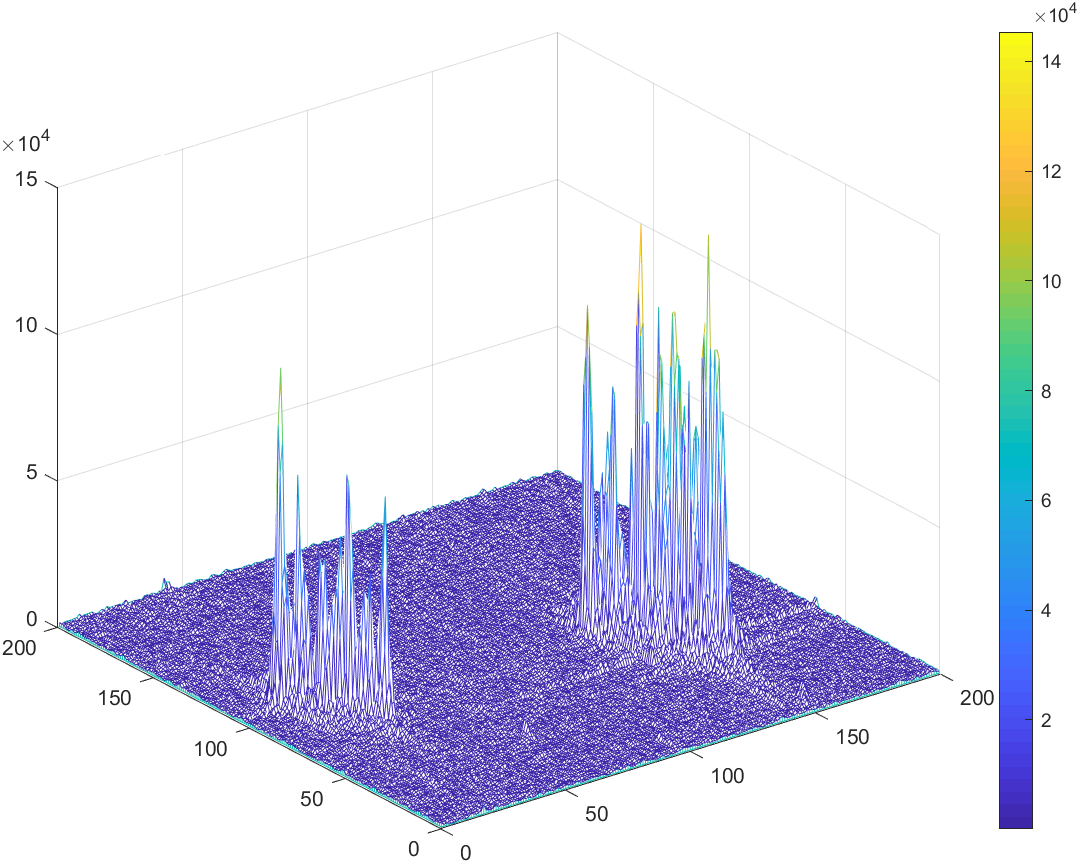
\includegraphics[width=9cm]{SPAN.png}}
    \caption{PCDNSPAN图像与SPAN图像对比}
    \label{fig:chap4:SPANCMP}
  \end{figure}

  图像检测结果,本次实验所使用的GPU为TiTAN V,运行显存内存为12G。基于MATLAB的串行算法运行的CPU为Intel(R) i7-9750H,系统内存为16G。
  为了验证检测结果的有效性,我们将PCDM方法与第二章实现的PWF方法进行对比如图\ref{fig:chap4:reultCMP}所示,从左到右依次为SPAN图像,PWF检测结果,PCDM检测结果。
  从检测结果上来看,PCDM得到的舰船检测结果与Pauli图像更加吻合,舰船边缘相较于PWF方法检测结果更加精确。算法的检测性能使用第二章定义的品质因数$F_1$来表示
  即正确检测数量与虚警数量和船只真实数量之和的比值。检测结果如表\ref{tab:chap4:detectresult}所示,PCDM的检测的品质因数高于PWF检测方法,可以得出结论PCDM算法对于
  复杂海况的适应能力比PWF强,即使面对不同海况依然可以保持高检测精度。

  在PCDM方法中不需要使用大量的海杂波像素去估计滤波器参数,该算法主要是计算大小为3x3的极化协方差差异矩阵及其特征值,因此算法在时间与空间性能上都优于极化白化滤波器方法。
  CPU串行与GPU并行的PCDM算法时间如表所示,因为GPU设备初始化开销代价所占比重较大,且CPU与GPU之间需要进行数据拷贝、通信与同步,所以本身在CPU上运行时间较短的程序在GPU上
  的加速比会降低。对于大小为1000x1000的SAR图像,经过多次实验测试,并行PCDM算法在Titan V上的运行的平均时间为0.69s,串行MATLAB方法在CPU上的运行时间为11.37秒,在时间性能上
  获得了近17倍的提升。

  
  \begin{figure}[h]
    \centering
    \subcaptionbox{SPAN图\label{chap4:fig:subfig2}}
        {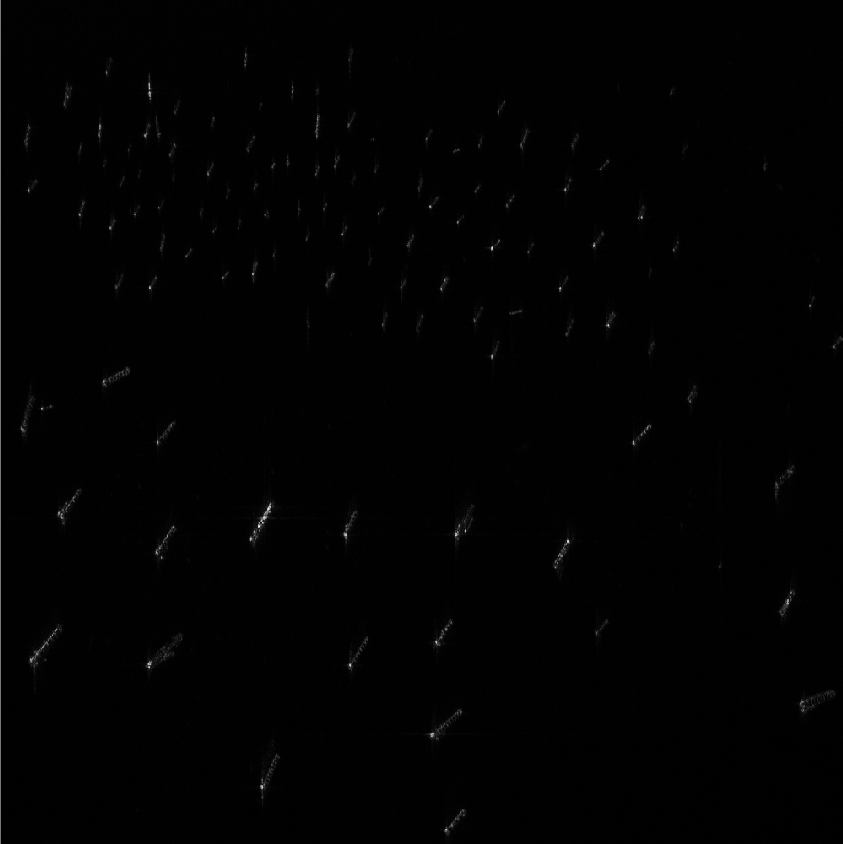
\includegraphics[width=7cm]{resultSPAN.png}}
    \subcaptionbox{PWF检测结果\label{chap4:fig:subfig2}}
        {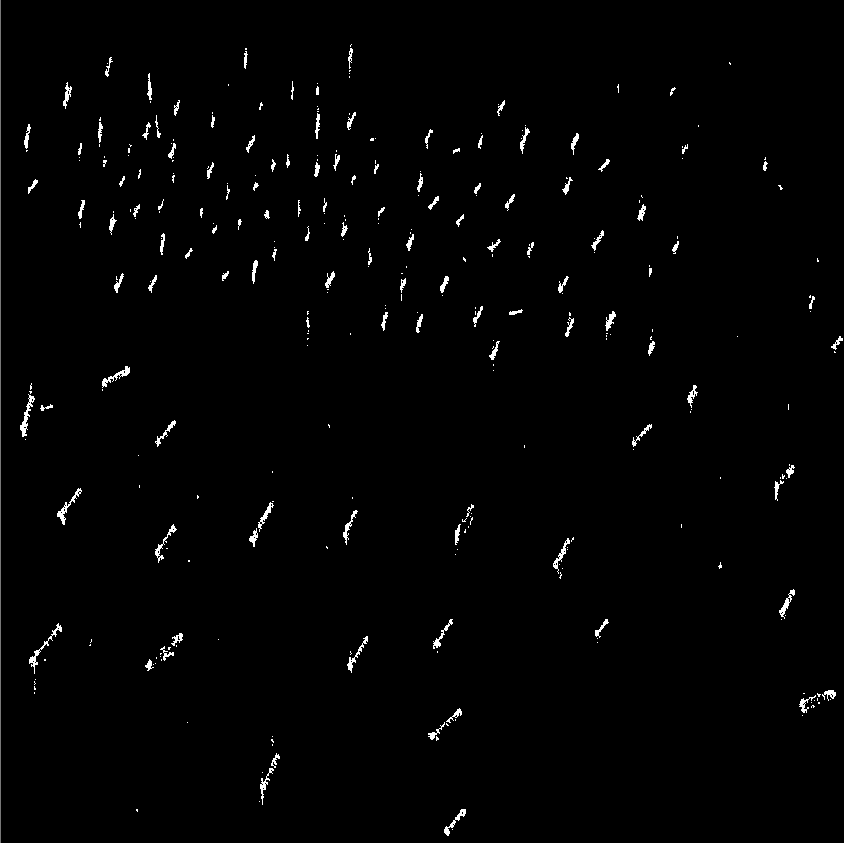
\includegraphics[width=7cm]{resultPWF.png}}

    \subcaptionbox{PCDM检测结果}
        {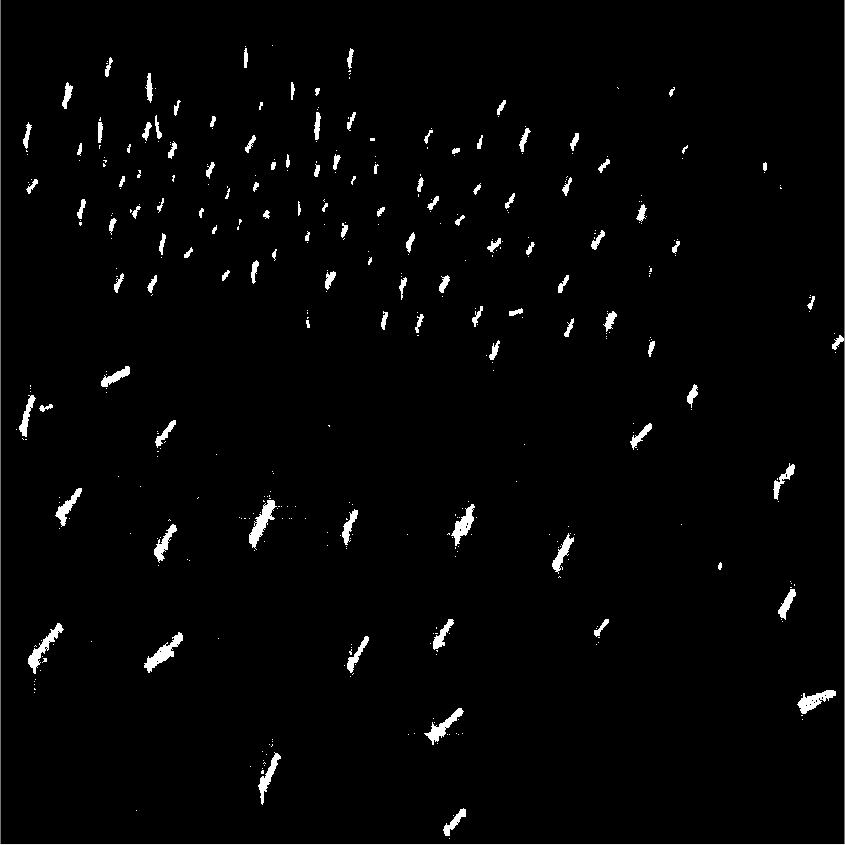
\includegraphics[width=7cm]{resultPCDM.png}}    
    \caption{舰船检测结果(a)SPAN图像;(b)PWF;(c)PCDM}
    \label{fig:chap4:reultCMP}
  \end{figure}

  \begin{table}[htb]
  \centering
    \begin{minipage}[t]{1\linewidth} % 如果想在表格中使用脚注,minipage是个不错的办法
    \caption[PCDM检测结果]{SAR图像检测结果对比}
    \label{tab:chap4:detectresult}
      \begin{tabularx}{\linewidth}{lXXXXXX}
        \toprule[1.5pt]
        {\heiti 检测方法} & {\heiti 船只数量} & {\heiti 总检测数量} & {\heiti 正确检测数量} & {\heiti 虚警数量} & {\heiti 漏报数量} & {\heiti $F_1$}\\ \midrule[1pt]
        PCDM & 118 & 120 & 117 & 3 & 1 & 0.967 \\
        PWF & 118 & 123 & 117 & 6 & 1 & 0.943 \\
        \bottomrule[1.5pt]
      \end{tabularx}
    \end{minipage}
\end{table}

  \begin{table}[htb]
  \centering
    \begin{minipage}[t]{1\linewidth} % 如果想在表格中使用脚注,minipage是个不错的办法
    \caption[PCDM算法运行时间对比]{不同平台算法运行时间对比}
    \label{tab:chap4:timeresult}
      \begin{tabularx}{\linewidth}{lXX}
        \toprule[1.5pt]
      {\heiti 检测算法} & {\heiti 运行平台} & {\heiti 运行时间/s} \\ \midrule[1pt]
        PCDM(MATLAB) & (Intel(R) i7-9750H CPU) & 11.4\\
        GPU并行PCDM & GPU(Titan V) & 0.67 \\
        PWF(C++) & (Intel(R) i9-7920X CPU) & 67.4\\
        GPU多线程PWF &  GPU(Titan V) & 2.1 \\
        多卡协同PWF & 2 GPU(Titan V) & 1.27 \\
        \bottomrule[1.5pt]
      \end{tabularx}
    \end{minipage}
\end{table}

\section{小结}
    对于极化SAR图像中的舰船目标检测,在本章我们实现了基于极化协方差差异矩阵的舰船检测方法。在该方法中,
    类比于光学图像检测中的LBP特征,我们引出了极化SAR图像的极化协方差差异矩阵(PCDM)的概念,PCDM矩阵计算了
    待检测像素与邻域像素的协防差矩阵差异,充分利用了空间相干信息,提高了舰船目标与背景杂波之间的对比度。
    接下来我们将PCDM矩阵应用于舰船检测,首先使用PCDM矩阵的SPAN值对船海像素做了一个粗略的划分,然后提取了PCDM矩阵
    的PSH极化特征,将该特征用于舰船目标检测,最后联合SPAN检测器得到的初步检测结果得到了最终的检测结果。实验结果
    表明PCDM方法可以有效的适应不同的复杂海况,相较于PWF算法,在检测精度、时间与空间消耗上都优于PWF算法。最后我们
    实现了基于GPU的并行PCDM方法,将图像像素对应的PCDM矩阵与PSH极化特征计算对应到每一个GPU线程中去并发执行。相比于
    串行执行的方式,并行的方法在时间性能上提升了近20倍,可以满足实时检测的要求



\chapter{总结与展望}
本文针对极化SAR图像目标检测算法中存在的计算量大,耗时长等问题提出了基于CPU+GPU异构架构的解决方案。
本文详细的分析了几种典型的基于分布和基于极化分解的SAR图像舰船检测方法,并分离其中可并行执行的部分,实现了基于
GPU的并行SAR图像舰船检测方法,本文完成的工作和创新点主要包括:

1)实现了基于GPU的极化白化滤波器极化SAR舰船目标检测算法,采用GPU多线程并行计算滑动窗内海杂波对应的
极化白化滤波器参数,并计算分割阈值得到检测结果。此外还合理的将数据与任务分配到了多块GPU上同时并行
计算,使得算法在时间效率进一步提升。2)实现了基于GPU的LMM舰船检测方法,该算法将估计海杂波分布参数的部分
附加到GPU上执行,并对参数迭代的过程使用GPU共享内存进行优化,实验结果表明基于GPU的LMM算法在时间性能上获得了数十倍的提升。
3)实现了基于GPU的PCDM舰船检测方法,该算法将PCDM矩阵与提取PCDM矩阵极化特征的计算部分放在GPU上并行计算。并行算法在
检测时间效率上获得了数十倍的提升,并且对复杂海况具有很好适应性。

本文在基于GPU的极化SAR图像检测上取得一定的成果,但是受限于时间、数据等原因,未来的工作还可以在以下几个方面展开:

1)在PCDM检测方法中,本文对于极化协方差差异矩阵的SPAN值与PSH特征采用经验阈值进行分割,可以尝试对这两个极化特征进行统计分析
以得到更加精准的自适应阈值,从而提升算法的检测精度。2)受限于CUDA提供的MATH API,较难实现Gamma分布,K分布等其它海杂波统计
模型,之后可以探究可在GPU上运算的更多统计分布模型,从而对海杂波分布拟合结果更加精准。3)算法基于linux系统下的CUDA运行环境进行设计,
并没有针对SAR系统实际的硬件环境来设计,未来可以结合含有嵌入式的GPU的SAR图像处理系统对算法在接口,时间,内存,功耗上做进行进一步的优化。



%%% 其它部分
\backmatter

%% 本科生要这几个索引,研究生不要。选择性留下。
% 插图索引
\listoffigures
% 表格索引
\listoftables
% 公式索引
\listofequations


%% 参考文献
% 注意:至少需要引用一篇参考文献,否则下面两行可能引起编译错误。
% 如果不需要参考文献,请将下面两行删除或注释掉。
\bibliographystyle{thuthesis-numeric}      % 顺序编码制
% \bibliographystyle{thuthesis-author-year}  % 著者-出版年制
%\bibliographystyle{thuthesis-bachelor}     % 本科生参考文献的著录格式
\bibliography{ref/refs}


%% 致谢
% 如果使用声明扫描页,将可选参数指定为扫描后的 PDF 文件名,例如:
% \begin{acknowledgement}[scan-statement.pdf]
\begin{acknowledgement}
  衷心感谢我的导师杨健教授在本次毕业设计中对我的精心指导和帮助。杨老师是我的班主任,这四年的大学生活中
  他在学习与科研工作等方面对我提出了很多针对性的建议和帮助。进入实验室的这一年时间,在与老师与学长的交流中,我的学术
  科研能力获得了很大的提升。

  感谢金侃、王洪淼、林惠平、朱庆涛、陈航、张涛等师兄对我毕业设计的指导和帮助,当我面临算法设计上的困难时
  感谢你们的建议让我获得了获得了更多的知识与更宽广的设计思路。

  感谢我的父母,感谢他们一直的辛勤付出与支持。因为疫情,此次毕设大部分工作都在家中完成,感谢他们这
  段时间在生活上的对我的关心与照料。

\end{acknowledgement}


%% 附录
\begin{appendix}

\chapter{外文资料的调研阅读报告或书面翻译}

\title{基于变分贝叶斯推断的极化SAR舰船检测}

{\heiti 摘要:在本文中,我们创新的提出了一种基于变分贝叶斯推断的极化SAR图像舰船检测方法。首先我们将极化SAR图像
表示为一个张量,并且将SAR图像分解为与舰船有关的稀疏分量和海杂波分量的总和。这些成分由一些潜在变量表示。之后我们介绍了
潜在变量的层次先验并建立了舰船检测的概率模型。通过变分贝叶斯推断的方法,我们计算得到潜变量的后验分布。最后在迭代贝叶斯推断
过程中获得舰船检测结果。本文提出的方法采用张量的形式表示极化SAR图像,显式的使用了SAR图像所有通道的极化信息从而避免了采用标量极化特征
表示可能导致的信息丢失。此外本文提出的方法不需要使用滑动窗,变分贝叶斯推断过程实际上使用了所有的像素而不是滑动窗内有限的像素,
因此该方法具有良好的舰船检测性能和目标形状保持能力,适用于拥挤海域的舰船检测。本次实验采用了C波段radarsat-2极化SAR数据,实验结果表明方法可以
实现最先进的舰船检测性能。}

\section{介绍}
基于SAR图像的舰船检测在渔业、海上交通服务与海上安全等领域都有十分重要的应用。相较于传统的单极化SAR舰船检测,
极化信息的加入可以显著提升舰船检测结果的精度。举例来讲,在仅使用交叉极化通道(HV)的SAR图像检测中,在入射角为陡峭和中等的条件下可以
获得令人满意的结果,而同极化(HH或VV)需要更大角度入射角才能表现的较好。这些方法都不需要要复杂的极化信息融合方法。

对于多通道SAR图像,通常设计一个标量特征来增强船海对比度,然后将全局阈值或恒虚警率检测器应用于该标量特征。CFAR检测测通常使用滑动窗来
估计局部海杂波参数,然后根据虚警率计算分割像素值。类似单极化SAR舰船检测中的图像强度。散射总功率SPAN(散射矩阵F范数的平方)被自然的作为极化特征。
更多复杂的极化特征设计实质上都是极化信息融合方法,这些方法可以大致分为两大类,基于单视散射矩阵与基于多视协方差矩阵或相干矩阵的方法。
对于第一类,Yeremy通过使用Cameron分解实现了舰船检测。Touzi提出了基于堆成散射特性的方法。Nunziata使用共极化与交叉极化通道散射相关性来检测船只。
Novak提出了极化白化滤波器,通过融合散射矩阵的各个元素来生成一幅相干斑抑制图像。尽管这些方法在足够大的信杂比(SCR)的条件下检测效果较好,但他们更容易受到
变电噪声的影响,从而增加小型舰船的虚警率。对于第二类,Yang提出了广义优化极化对比增强(GOPCE)来最大化图像的信杂比。Chen介绍了基于极化相干矩阵分解的
极化交叉熵,并通过广义指数分布近似模拟海杂波的PCE值。Armando提出了一种基于几何扰动极化陷波滤波器(GP-PNF)的检测器,并推导了滤波值的概率密度分布函数。
Touzi使用极化度(Dop)和最小极化度的偏移来改善船海对比度。在这些方法中,通过空间整体平均来抑制斑点噪声,但是这种空域平均操作不利于
检测小型船只。

在多极化SAR舰船检测的实际应用中,上述提到的标量特征CFAR检测器有两个缺点:1)尽管标量隐含了不同通道的贡献,但是显示使用所有极化通道应该
可以提供更多的信息,而标量标识没有有效利用它。另外特征标量的理论分布较难分析,或者估计分布参数及其复杂。2)在多目标情况下,尤其是在
拥挤的海域,不适合的滑动窗大小将会导致对海杂波分布参数的错误估计,因此舰船检测性能将会下降。尽管顺序统计与其他的检测方法被提出来解决这一问题,但在
实践中仍然存在很多困难,例如先验依赖,计算复杂,应用场景限制等。

为了克服这些缺点,我们提出同时利用海面的低秩特性与舰船的稀疏特性。我们采用多维广义低秩模型和鲁棒主成分分析进行极化SAR图像舰船检测。
尽管在这些方法中没有使用极化数据融合与滑动窗,但是海平面的低秩特性是一个太严格的约束限制了这些方法的实际应用。因此在单极化SAR舰船
检测中,我们去除了低秩约束的限制仅利用了舰船的稀疏特性并采用了变分贝叶斯推断的方法用于SAR图像舰船检测,该方法实现了最先进的舰船检测性能。为了进一步处理多通道
SAR图像舰船检测并充分利用极化信息,在IEEE IGARSS 2016中我们提出将极化SAR图像与变分贝叶斯推断相结合。在本文中我们将提供有关该方法的更多详细信息,并
将其与最新的舰船检测方法进行比较以证明其有效性。因此本文是第一个正式致力于使用变分贝叶斯推断进行极化SAR图像舰船检测的工作。首先我们将多通道的极化SAR图像表示为
张量,并介绍了与之相关的多维变量的先验分布。因此我们没有应用极化信息融合而是提出了一个应用变分贝叶斯推断进行极化SAR图像舰船检测的通用框架。
其次我们进一步改善了舰船检测的概率模型,减少了隐变量的个数,简化了变分贝叶斯推断的过程。

本文的其余部分安排如下。第二章介绍了极化SAR图像中舰船检测的精准概率模型。第三节详细介绍了将变分贝叶斯推断应用于舰船检测。
第四节报告了实验结果。第五部分总结了本文的工作。

\section{极化SAR图像概率模型}
此前我们提出了单通道SAR图像的舰船检测概率模型。在本文中,我们将此基本模型扩展到极化SAR图像。我们将极化SAR图像定义为张量进而完善了此前提出的原始概率模型并引入适用的多元隐变量先验分布。
\subsection{极化SAR图像的表示}
对于单极化SAR图像,像素值由图像强度定义。对于全极化单视复图像,像素的复散射矢量在非互易的条件下定义如\ref{equ:append:repre}
所示。
\begin{equation}
    \label{equ:append:repre}
    \begin{array}{*{20}{c}}
    {{\bf{w}} = {{\left[ {\begin{array}{*{20}{c}}
    {{S_{HH}}}&{{S_{HV}}}&{{S_{VH}}}&{{S_{VV}}}
    \end{array}} \right]}^T}}&{{\rm{linear\ basis}}}\\
    {{\bf{w}} = \frac{1}{{\sqrt 2 }}\left[ {\begin{array}{*{20}{c}}
    {{S_{HH}} + {S_{VV}}}&{{S_{HH}} - {S_{VV}}}&{{S_{HV}} + {S_{VH}}}&{j({S_{HV}} - {S_{VH}})}
    \end{array}} \right]}&{{\rm{Pauli\ basis}}}
    \end{array}
\end{equation}

其中$S_{HH}$,$S_{HV}$,$S_{VH}$,$S_{VV}$定义了水平-垂直基下的散射矩阵元素。上标T为转置。在满足互易的情形下如式\ref{equ:append:reciprocal}所示
\begin{equation}
    \label{equ:append:reciprocal}
    \begin{array}{*{20}{c}}
    {{\bf{w}} = {{\left[ {\begin{array}{*{20}{c}}
    {{S_{HH}}}&{\sqrt 2 {S_{HV}}}&{{S_{VV}}}
    \end{array}} \right]}^T}}&{{\rm{linear basis}}}\\
    {{\bf{w}} = \frac{1}{{\sqrt 2 }}\left[ {\begin{array}{*{20}{c}}
    {{S_{HH}} + {S_{VV}}}&{{S_{HH}} - {S_{VV}}}&{2{S_{HV}}}
    \end{array}} \right]}&{{\rm{Pauli basis}}}
    \end{array}
\end{equation}

在这里,我们进一步将复散射矢量$\bf{w}$表示为实向量$\bf{d}$的形式,如式\ref{equ:append:realvector}所示。其中$d$为三或四对应互易或者非互易的情形。
\begin{equation}
    \label{equ:append:realvector}
   {\bf{d}} = \left[ {{\mathop{\rm Re}\nolimits} ({{\bf{w}}_{\bf{1}}}){\mathop{\rm Im}\nolimits} ({{\bf{w}}_{\bf{1}}}) \ldots {\mathop{\rm Re}\nolimits} ({{\bf{w}}_d}){\mathop{\rm Im}\nolimits} ({{\bf{w}}_d})} \right] 
\end{equation}

在SAR图像中,海杂波像素值是随机变化的,舰船显示为稀疏分布的目标像素具有显著的稀疏特征。因此使用张量术语我们可以将舰船
检测视为从海杂波中恢复稀疏信号的问题,其中采用张量表示的极化SAR图像可以被建模为
\begin{equation}
    \label{equ:append:construct}
    {\bf{D = A*S + C}}
\end{equation}

${\bf{D}} \in {\mathbb{R}^{m \times n \times 2d}}{\bf{A*S}} \in {\mathbb{R}^{m \times n \times 2d}}{\bf{C}} \in {\mathbb{R}^{m \times n \times 2d}}$分别代表SAR图像,严格稀疏的舰船成分,海杂波成分。
Tube fiber定义为有固定行列索引的实向量如式\ref{equ:append:realvector}的形式。${\bf{A}} \in {\mathbb{R}^{m \times n \times 2d}}$的所有正面切片均为相同的二进制数值矩阵${\bf{A}}{\rm{ = }}\left[ {{{\rm{a}}_{ij}}} \right] \in {\mathbb{R}^{m \times n}}$
其中第$(i,j)$个元素$a_{ij}=1$表示该像素为舰船像素。故将矩阵$\bf{A}$视为舰船检测结果。${\bf{S}} \in {\mathbb{R}^{m \times n \times 2{\rm{d}}}}$是非严格稀疏的舰船分量矩阵,$*$表示哈达玛积。在这我们定义$d_{ij:},s_{ij:},c_{ij:}$为张量${\bf{D,S,C}}$的tube fiber。

现在值得花一些时间去研究式\ref{equ:append:construct}的形式,因为它可以提供模型细化的一些观点。从式\ref{equ:append:construct}中我们可以看出当$a_{ij}=1$时,$d_{ij:}=s_{ij:}+c_{ij:}$。当$a_{ij}=0$时,$d_{ij:}=c_{ij:}$。因为舰船检测的目的是估计二进制潜变量$\bf{A}$
而不是$\bf{S}$,因此当$a_{ij}=1$时,我们可以进一步约束$c_{ij:}=\bf{0}$,因此$\bf{S}$实际上是$\bf{D}$,式\ref{equ:append:construct}可以表示为
\begin{equation}
   \label{equ:append:refine}
   {\bf{D = A*D + C}} 
\end{equation}

在本文中,我们使用这个改进的方法来表示SAR图像,并通过变分贝叶斯推断估计了隐变量$\bf{A}$与$\bf{C}$。相比于文献[21]中的分析,概率模型与变分贝叶斯推断的过程在本文中都进行了改进。为了提升模型对复杂场景中的稀疏舰船成分的检测能力,$a_{ij},c_{ij:}$的独立先验定义如下。
\subsection{稀疏分量$\bf{A}$的先验分布}
将二进制标记系数$a_{ij}$建模为相同的分布即
    \begin{equation}
        \label{equ:append:priora}
        \begin{array}{*{20}{c}}
        {{\rm{p}}({a_{ij}}|{e_{ij}}) = e_{ij}^{{a_{ij}}}{{(1 - {e_{ij}})}^{1 - {a_{ij}}}}}\\
        {P({e_{ij}}) = Beta({\alpha _0},{\beta _0})}
        \end{array}
    \end{equation}

其中$e_{ij}$代表了舰船像素的存在概率,$\alpha_0>0, \beta_0>0$为超参数。$\rm{Beta(\cdot)}$为Beta分布。
因此$e_{ij}$的期望$E(e_{ij})$为$\frac{{{\alpha _0}}}{{{\alpha _0} + {\beta _0}}}$并且$E(a_{ij})$接近0。在这种情形下,稀疏条件加于
$A$上。为了简化分析我们让${\alpha _0} \ll 0$并限制${\alpha _0}{\rm{ + }}{\beta _0} = 1$。需要注意的是$\alpha_0,\beta_0$并不依赖于其他参数并且他们被设置为确定性的值,下节的其他超参数也是如此。

\subsection{海杂波$\bf{C}$的先验分布}
\section{变分贝叶斯推断}
\section{实验与结果}
\section{结论}


\end{appendix}

%% 个人简历
%\begin{resume}

  \resumeitem{个人简历}

  xxxx 年 xx 月 xx 日出生于 xx 省 xx 县。

  xxxx 年 9 月考入 xx 大学 xx 系 xx 专业,xxxx 年 7 月本科毕业并获得 xx 学士学位。

  xxxx 年 9 月免试进入 xx 大学 xx 系攻读 xx 学位至今。

  \researchitem{发表的学术论文} % 发表的和录用的合在一起

  % 1. 已经刊载的学术论文(本人是第一作者,或者导师为第一作者本人是第二作者)
  \begin{publications}
    \item Yang Y, Ren T L, Zhang L T, et al. Miniature microphone with silicon-
      based ferroelectric thin films. Integrated Ferroelectrics, 2003,
      52:229-235. (SCI 收录, 检索号:758FZ.)
    \item 杨轶, 张宁欣, 任天令, 等. 硅基铁电微声学器件中薄膜残余应力的研究. 中国机
      械工程, 2005, 16(14):1289-1291. (EI 收录, 检索号:0534931 2907.)
    \item 杨轶, 张宁欣, 任天令, 等. 集成铁电器件中的关键工艺研究. 仪器仪表学报,
      2003, 24(S4):192-193. (EI 源刊.)
  \end{publications}

  % 2. 尚未刊载,但已经接到正式录用函的学术论文(本人为第一作者,或者
  %    导师为第一作者本人是第二作者)。
  \begin{publications}[before=\publicationskip,after=\publicationskip]
    \item Yang Y, Ren T L, Zhu Y P, et al. PMUTs for handwriting recognition. In
      press. (已被 Integrated Ferroelectrics 录用. SCI 源刊.)
  \end{publications}

  % 3. 其他学术论文。可列出除上述两种情况以外的其他学术论文,但必须是
  %    已经刊载或者收到正式录用函的论文。
  \begin{publications}
    \item Wu X M, Yang Y, Cai J, et al. Measurements of ferroelectric MEMS
      microphones. Integrated Ferroelectrics, 2005, 69:417-429. (SCI 收录, 检索号
      :896KM)
    \item 贾泽, 杨轶, 陈兢, 等. 用于压电和电容微麦克风的体硅腐蚀相关研究. 压电与声
      光, 2006, 28(1):117-119. (EI 收录, 检索号:06129773469)
    \item 伍晓明, 杨轶, 张宁欣, 等. 基于MEMS技术的集成铁电硅微麦克风. 中国集成电路,
      2003, 53:59-61.
  \end{publications}

  \researchitem{研究成果} % 有就写,没有就删除
  \begin{achievements}
    \item 任天令, 杨轶, 朱一平, 等. 硅基铁电微声学传感器畴极化区域控制和电极连接的
      方法: 中国, CN1602118A. (中国专利公开号)
    \item Ren T L, Yang Y, Zhu Y P, et al. Piezoelectric micro acoustic sensor
      based on ferroelectric materials: USA, No.11/215, 102. (美国发明专利申请号)
  \end{achievements}

\end{resume}


%% 本科生进行格式审查是需要下面这个表格,答辩可能不需要。选择性留下。
% 综合论文训练记录表
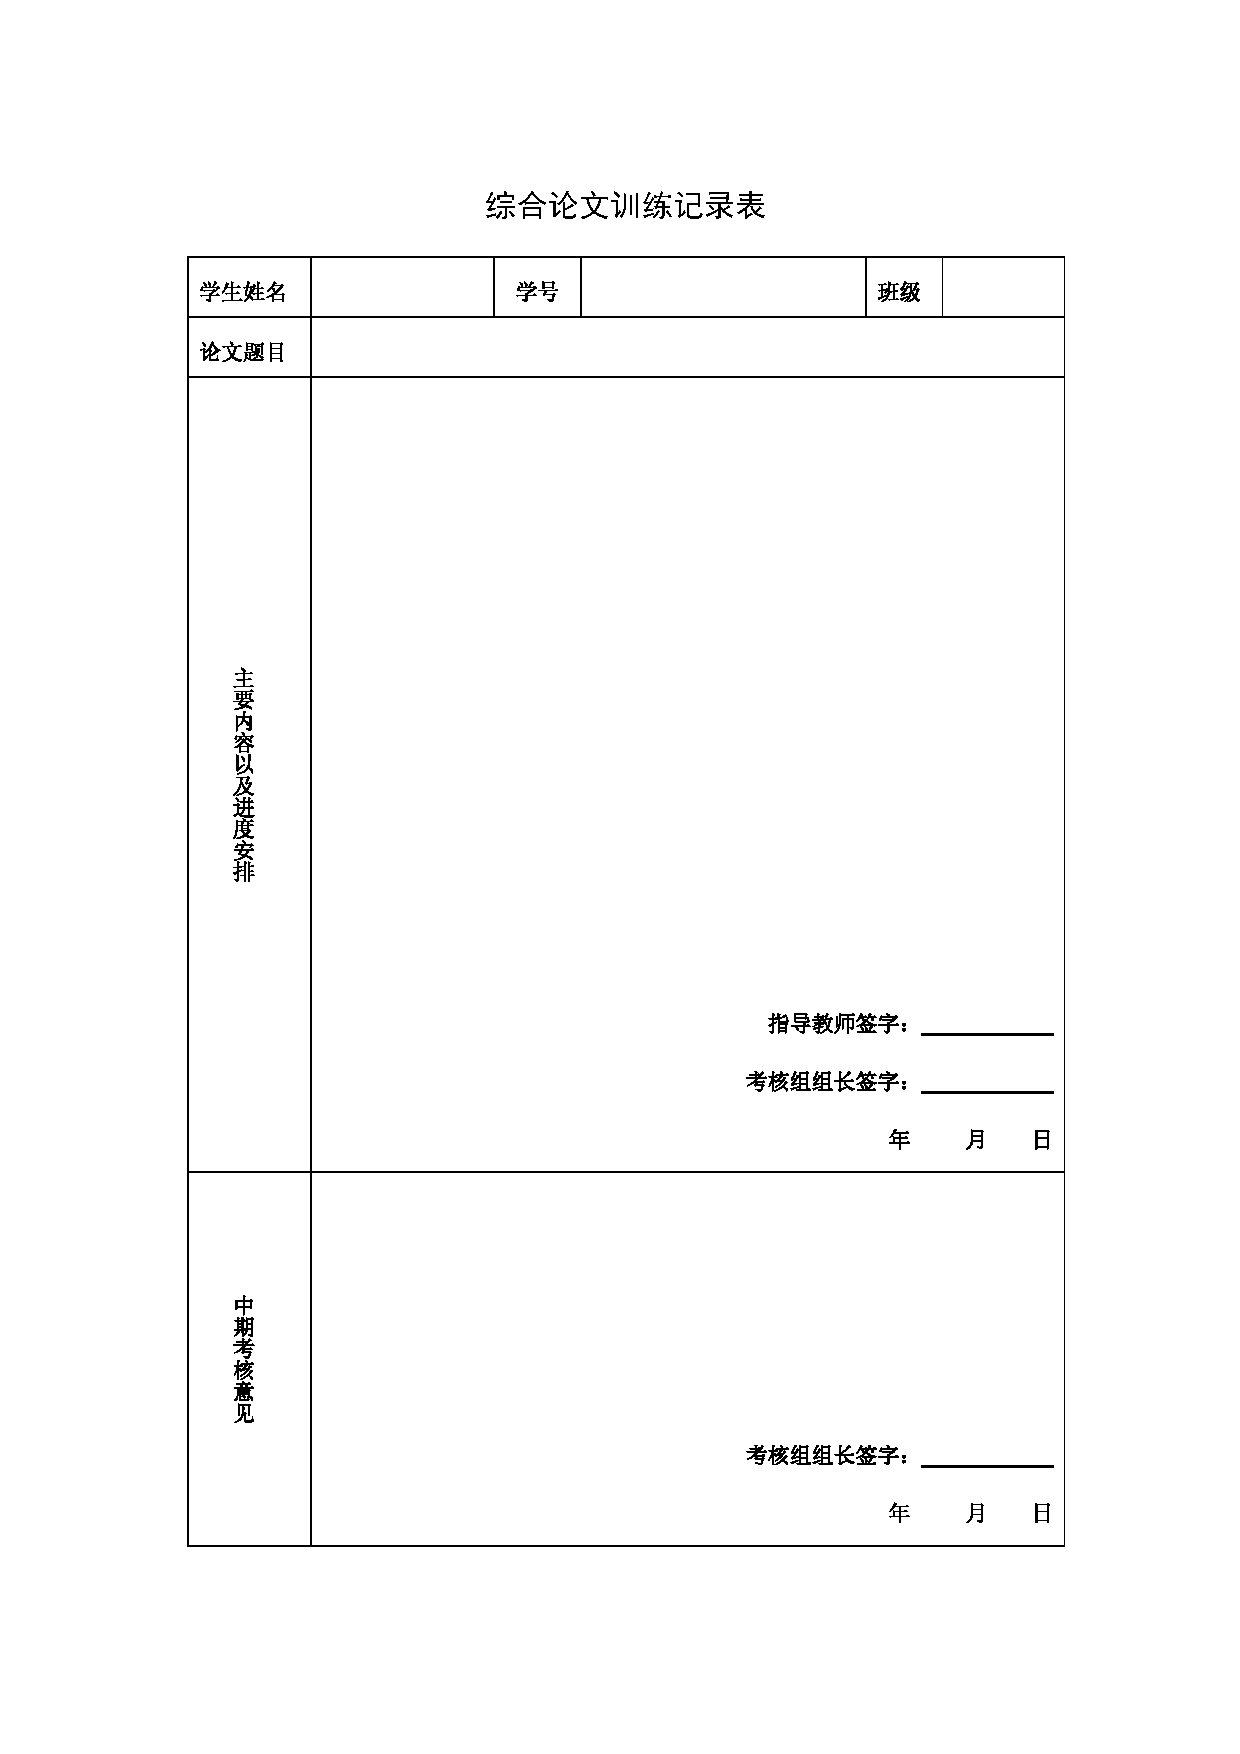
\includepdf[pages=-]{scan-record.pdf}
\end{document}
